\chapter{Appendix - User's guide}
\label{sec:usersGuide}

\section{Introduction}
This chapter describes some steps about how to use the application developed in details. Since the how to login to the system, the therapist actions and user actions.

\section{Web server application}
\label{sec:implwebserver}

The web server application\footnote{https://www.swheelchairth.com.br:8443/servletserver/} shown in Figure \ref{fig:apDmainFrontSite} was implemented using Java$\texttrademark$  Servlets and Multi-WebRTC framework and different channels to receive/redirect data. 

\begin{figure}[!hbt]
\begin{center}
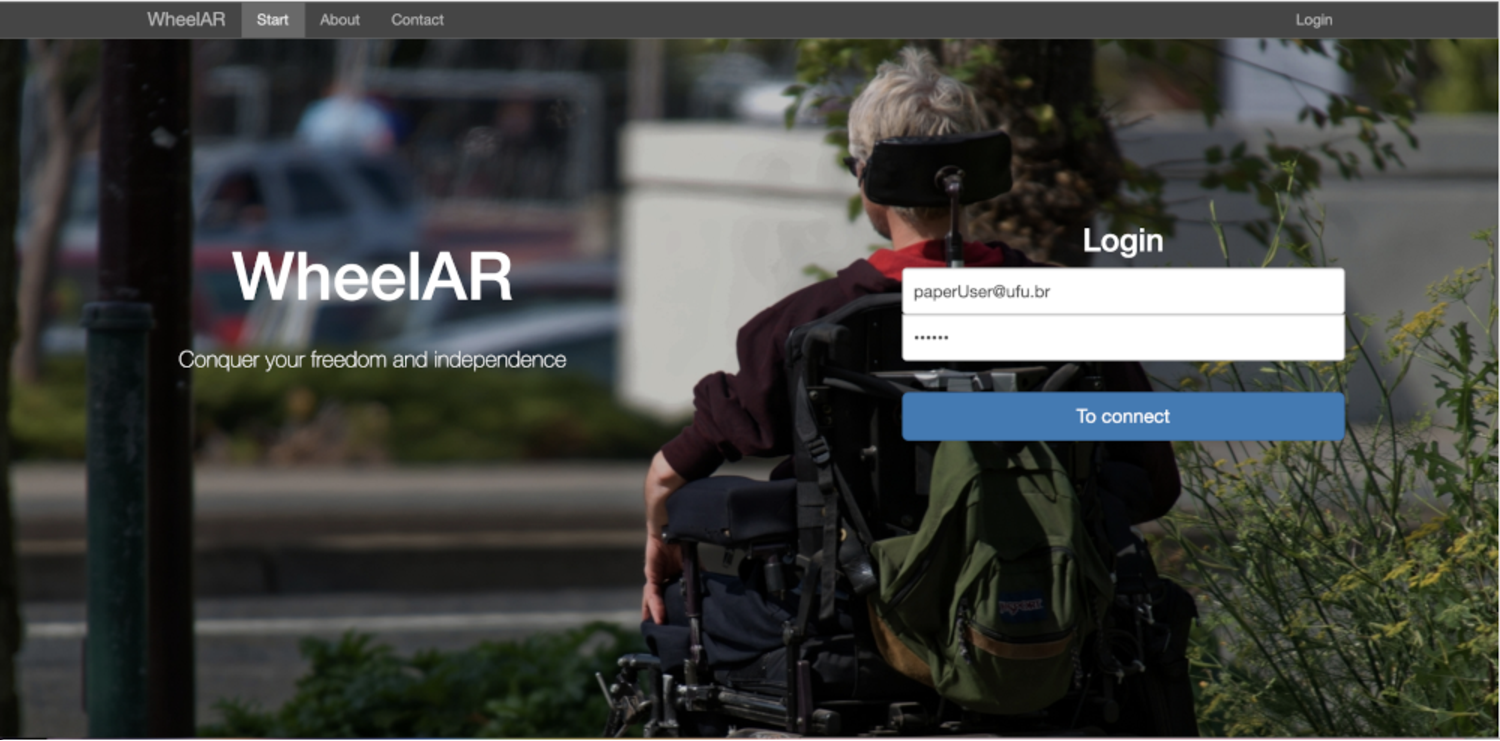
\includegraphics[width=1\linewidth]{img/apendiceD/mainFrontSite}
\caption{AR Wheel home page} \label{fig:apDmainFrontSite}
\end{center}
\end{figure}


Thus, the system platform is based on the MVC\cite{hansen2005}. This makes it easy to incorporate different libraries and frameworks (JSArtoolkit, Boostrap, Web Graphics Library (WebGL) and GL Transmission Format (GLTF) models) to build a reliable web application \cite{poltavskyi2020,zhou2019,mattioli2019,aquino2016}. Servlets are used in MVC model to control events that come from JSP page through POST, GET requests and also external data coming from sockets. In this system, there are two basic actors' roles: therapist and patient.

The following sections, explain the main implementation details about each site and respective session.

\subsection{Training site}
\label{sec:impltrainingsite}

The release to interact and visualize information of this environment by the user is given only by the therapist. 

The ``Start streaming'' is a web page that can be accessed from ``Begin session'' action inside the ``Define training'' menu. From the therapist desktop, a remote connection is established to the smartphone using the Team Viewer QuickSupport. Then, from a new therapist session the ``Define training'' menu is accessed and through the  ``Begin session'' action is redirected to the page shown in Figure \ref{fig:apDtStartStream}. Each new streaming (video/audio) session that is implemented over WebRTC API has an id randomly defined. When the  ``Start streaming'' button is pressed streaming is started. Thus, some updates are performed in order to lock the training site, change the patient status from  ``waiting'' to  ``training'', and a shared Uniform Resource Locator (URL) is also updated. Then the  ``Waiting page'' recognize this changes and redirect each user profile to respective ``ViewPort''.  After the training protocol is finished by the user, the therapist ends the video streaming pressing the  ``End call'' button, logout the web page and close the remote connection.

\begin{figure}[!hbt]
\begin{center}
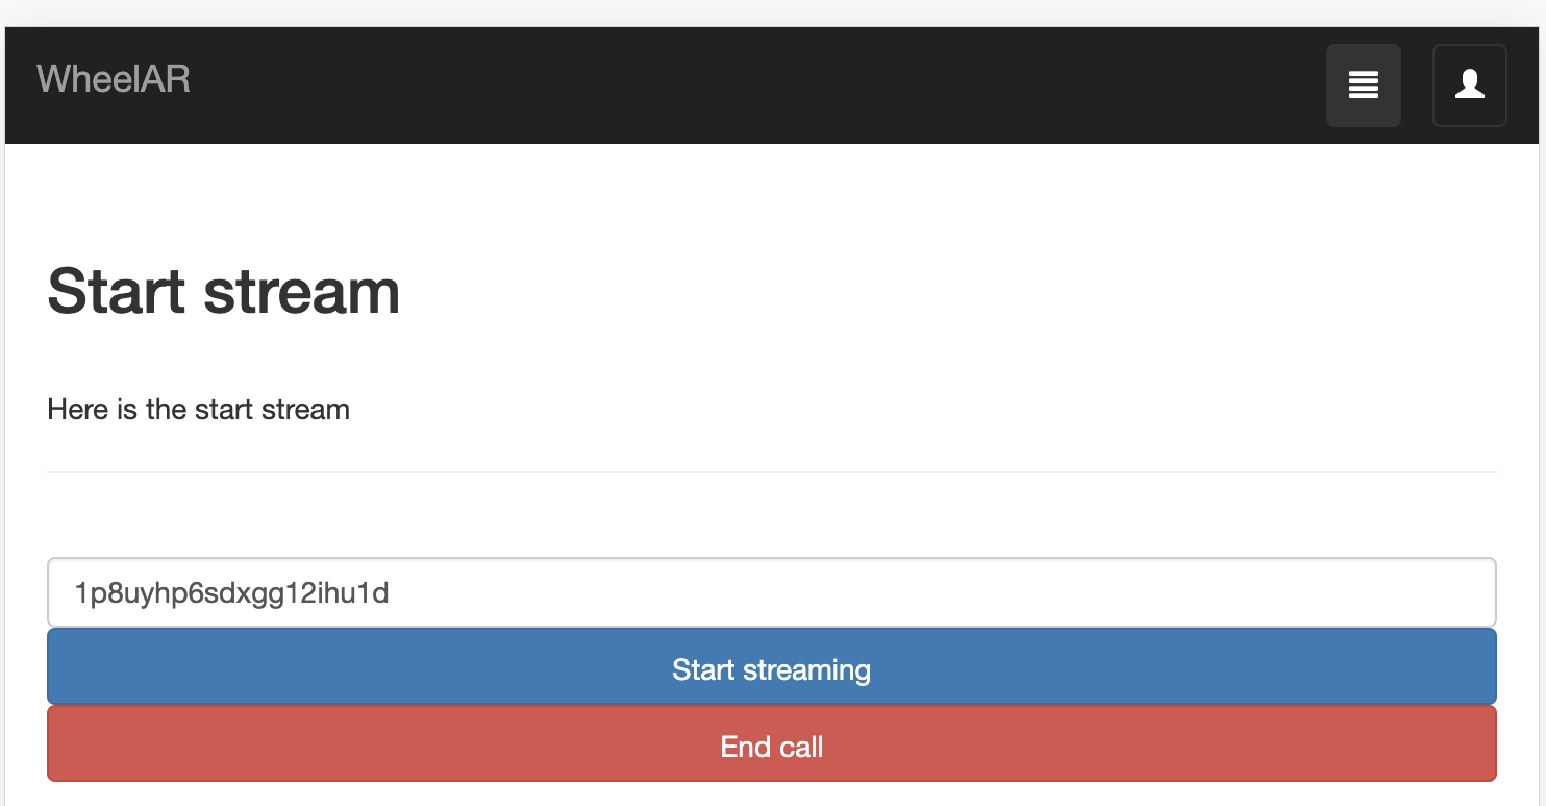
\includegraphics[width=0.5\linewidth]{img/apendiceD/tStartStream}
\caption{Start streaming therapist page} \label{fig:apDtStartStream}
\end{center}
\end{figure}

\subsection{Therapist session}
The menu sessions information is presented bellow:

\subsubsection{User register}

Used to register new patients and therapists as presented in Figure \ref{fig:apDtUserRegister}. According to the selected profile (therapist/patient) the system asks different information related to the user that will be stored into database. Some patients information asked are PW model, impairment time, health state (cognitive, visual and auditory) , ADL and AIVD performance and transport.

\begin{figure}[!hbt]
\begin{center}
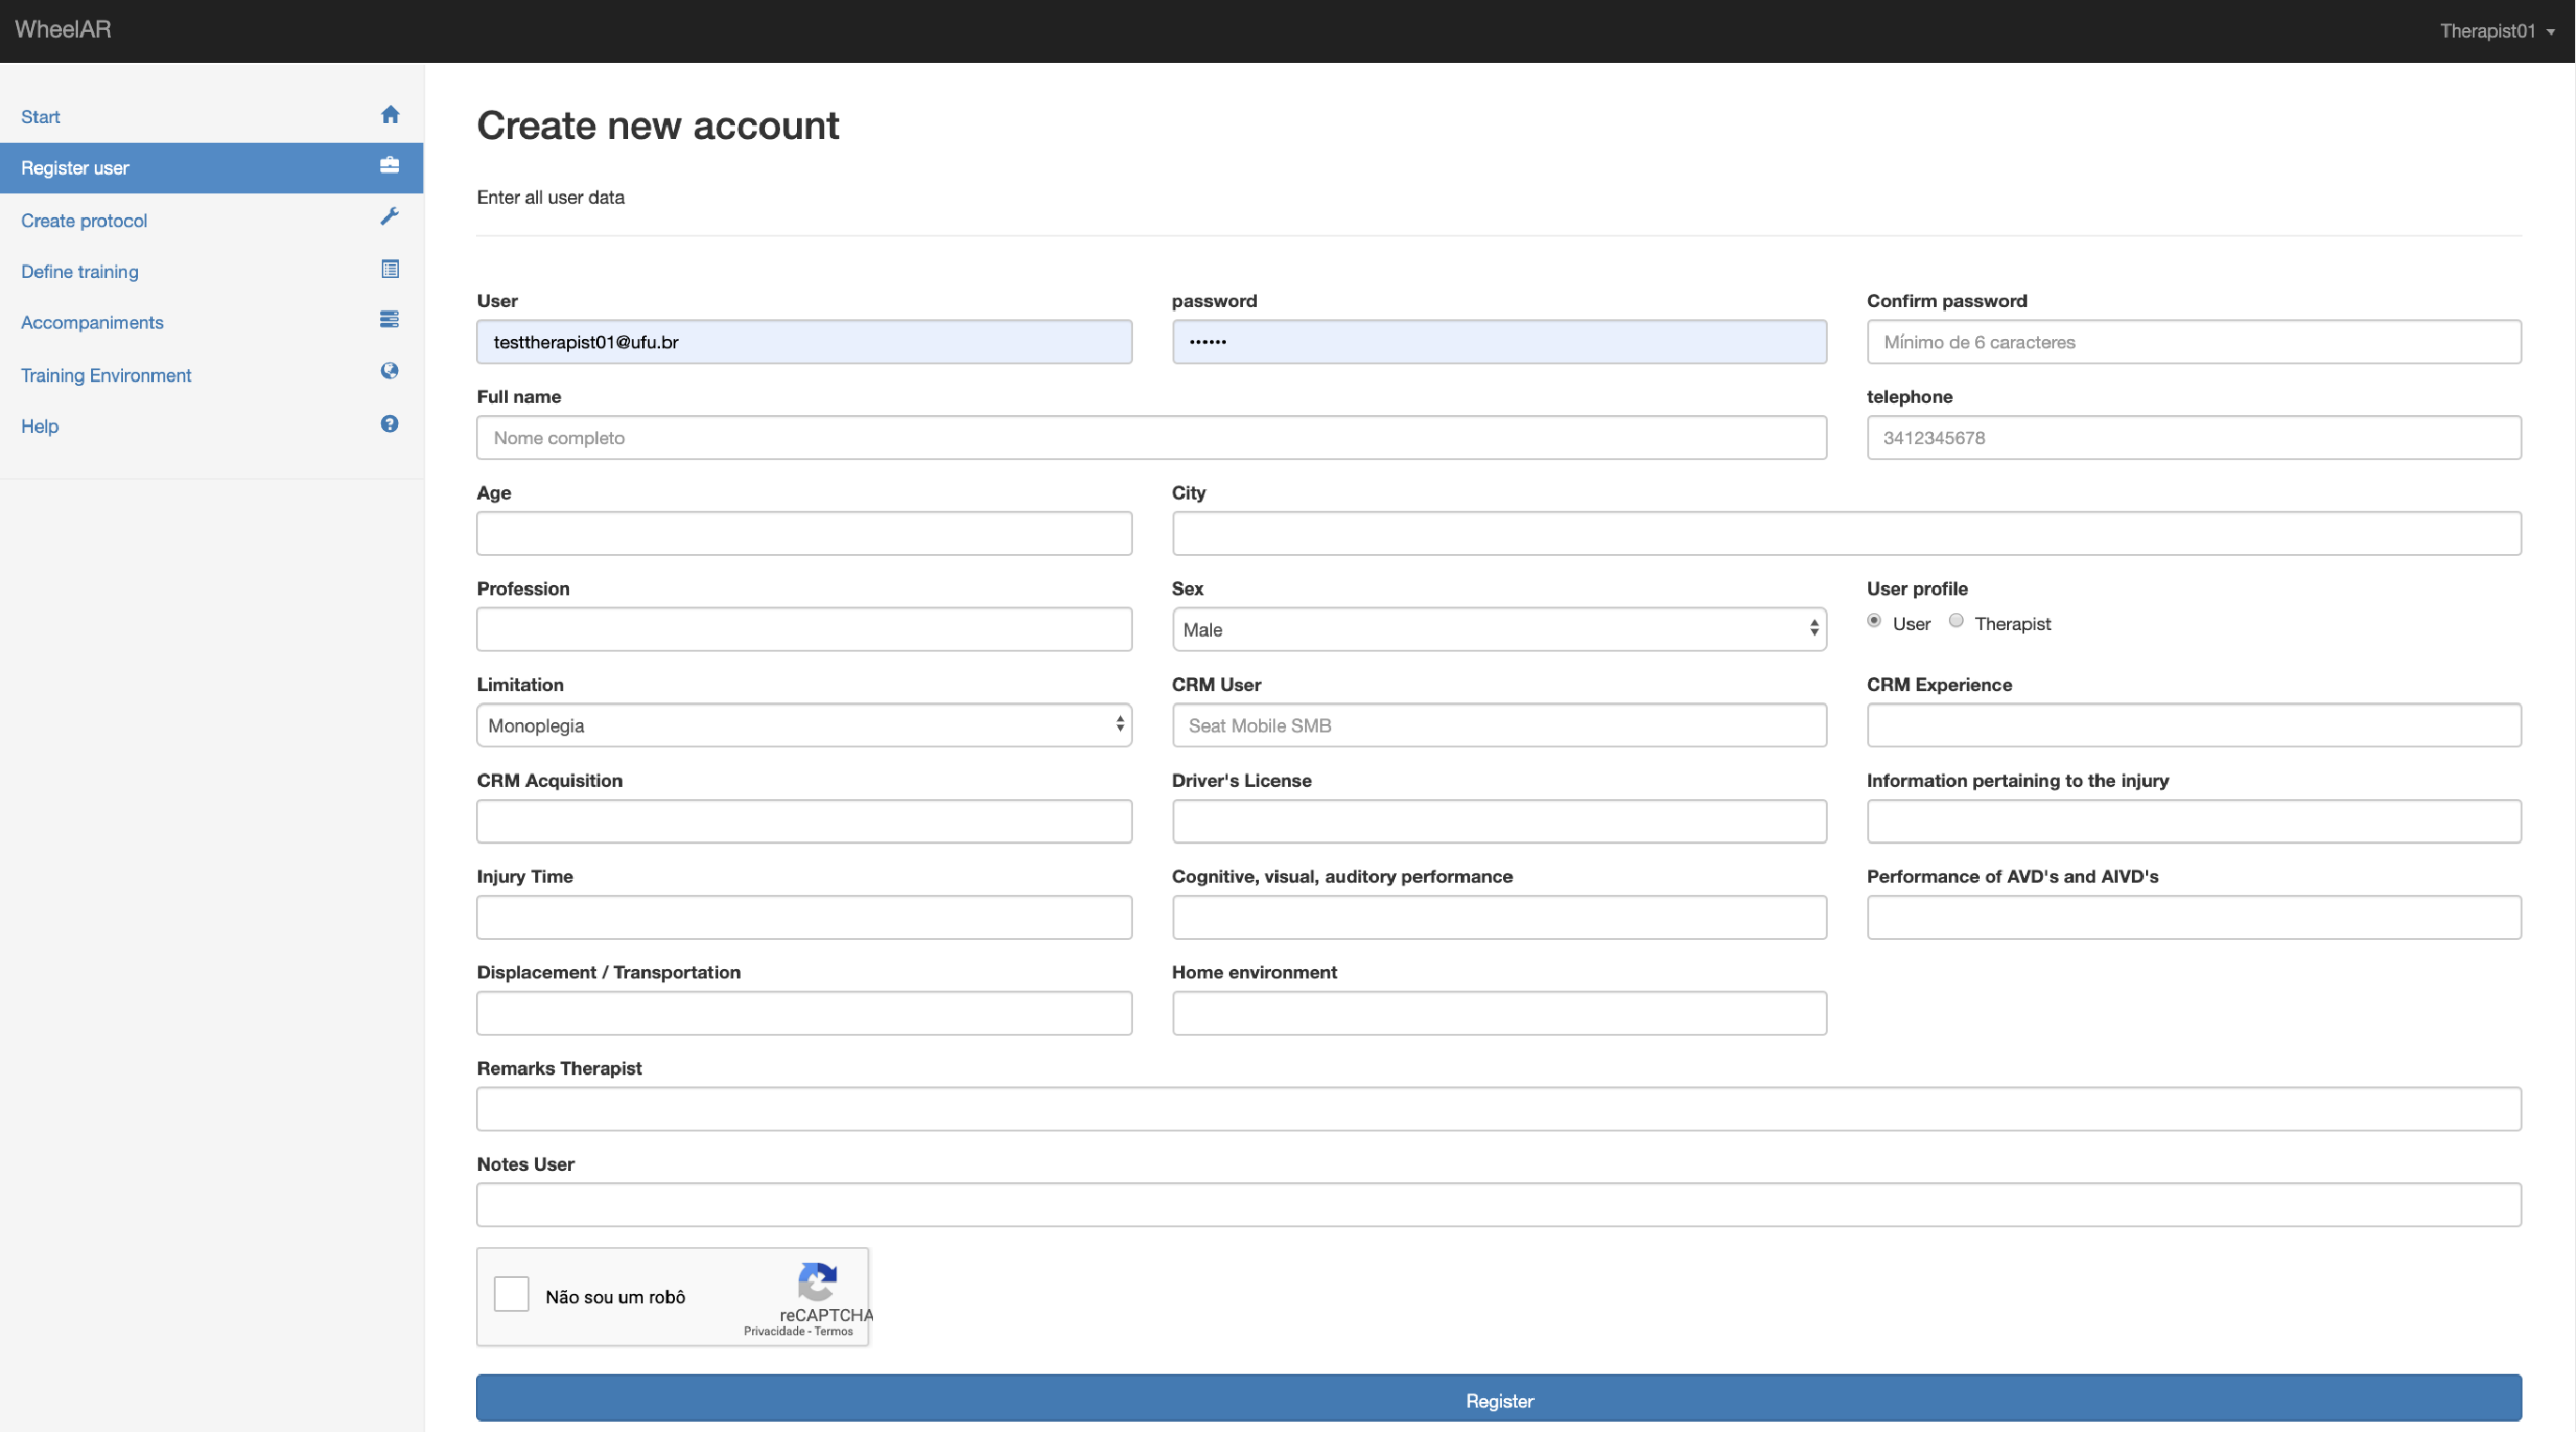
\includegraphics[width=0.95\linewidth]{img/apendiceD/tUserRegister}
\caption{Register a new user page} \label{fig:apDtUserRegister}
\end{center}
\vspace{-20pt}
\end{figure}

\subsubsection{Create protocol}
\label{sec:appCreateProcotol}

An adaptation of PMRT was implemented in order to allow the therapist to customise different  activities providing the user with their needs. The first step is to select all activities requested to the new protocol from ``Activities list'' clicking on ``Add activity'' to add or ``Clear activities'' clear all as presented on Figure \ref{fig:apDcreateProtocol01}. 

\begin{figure}[!hbt]
\begin{center}
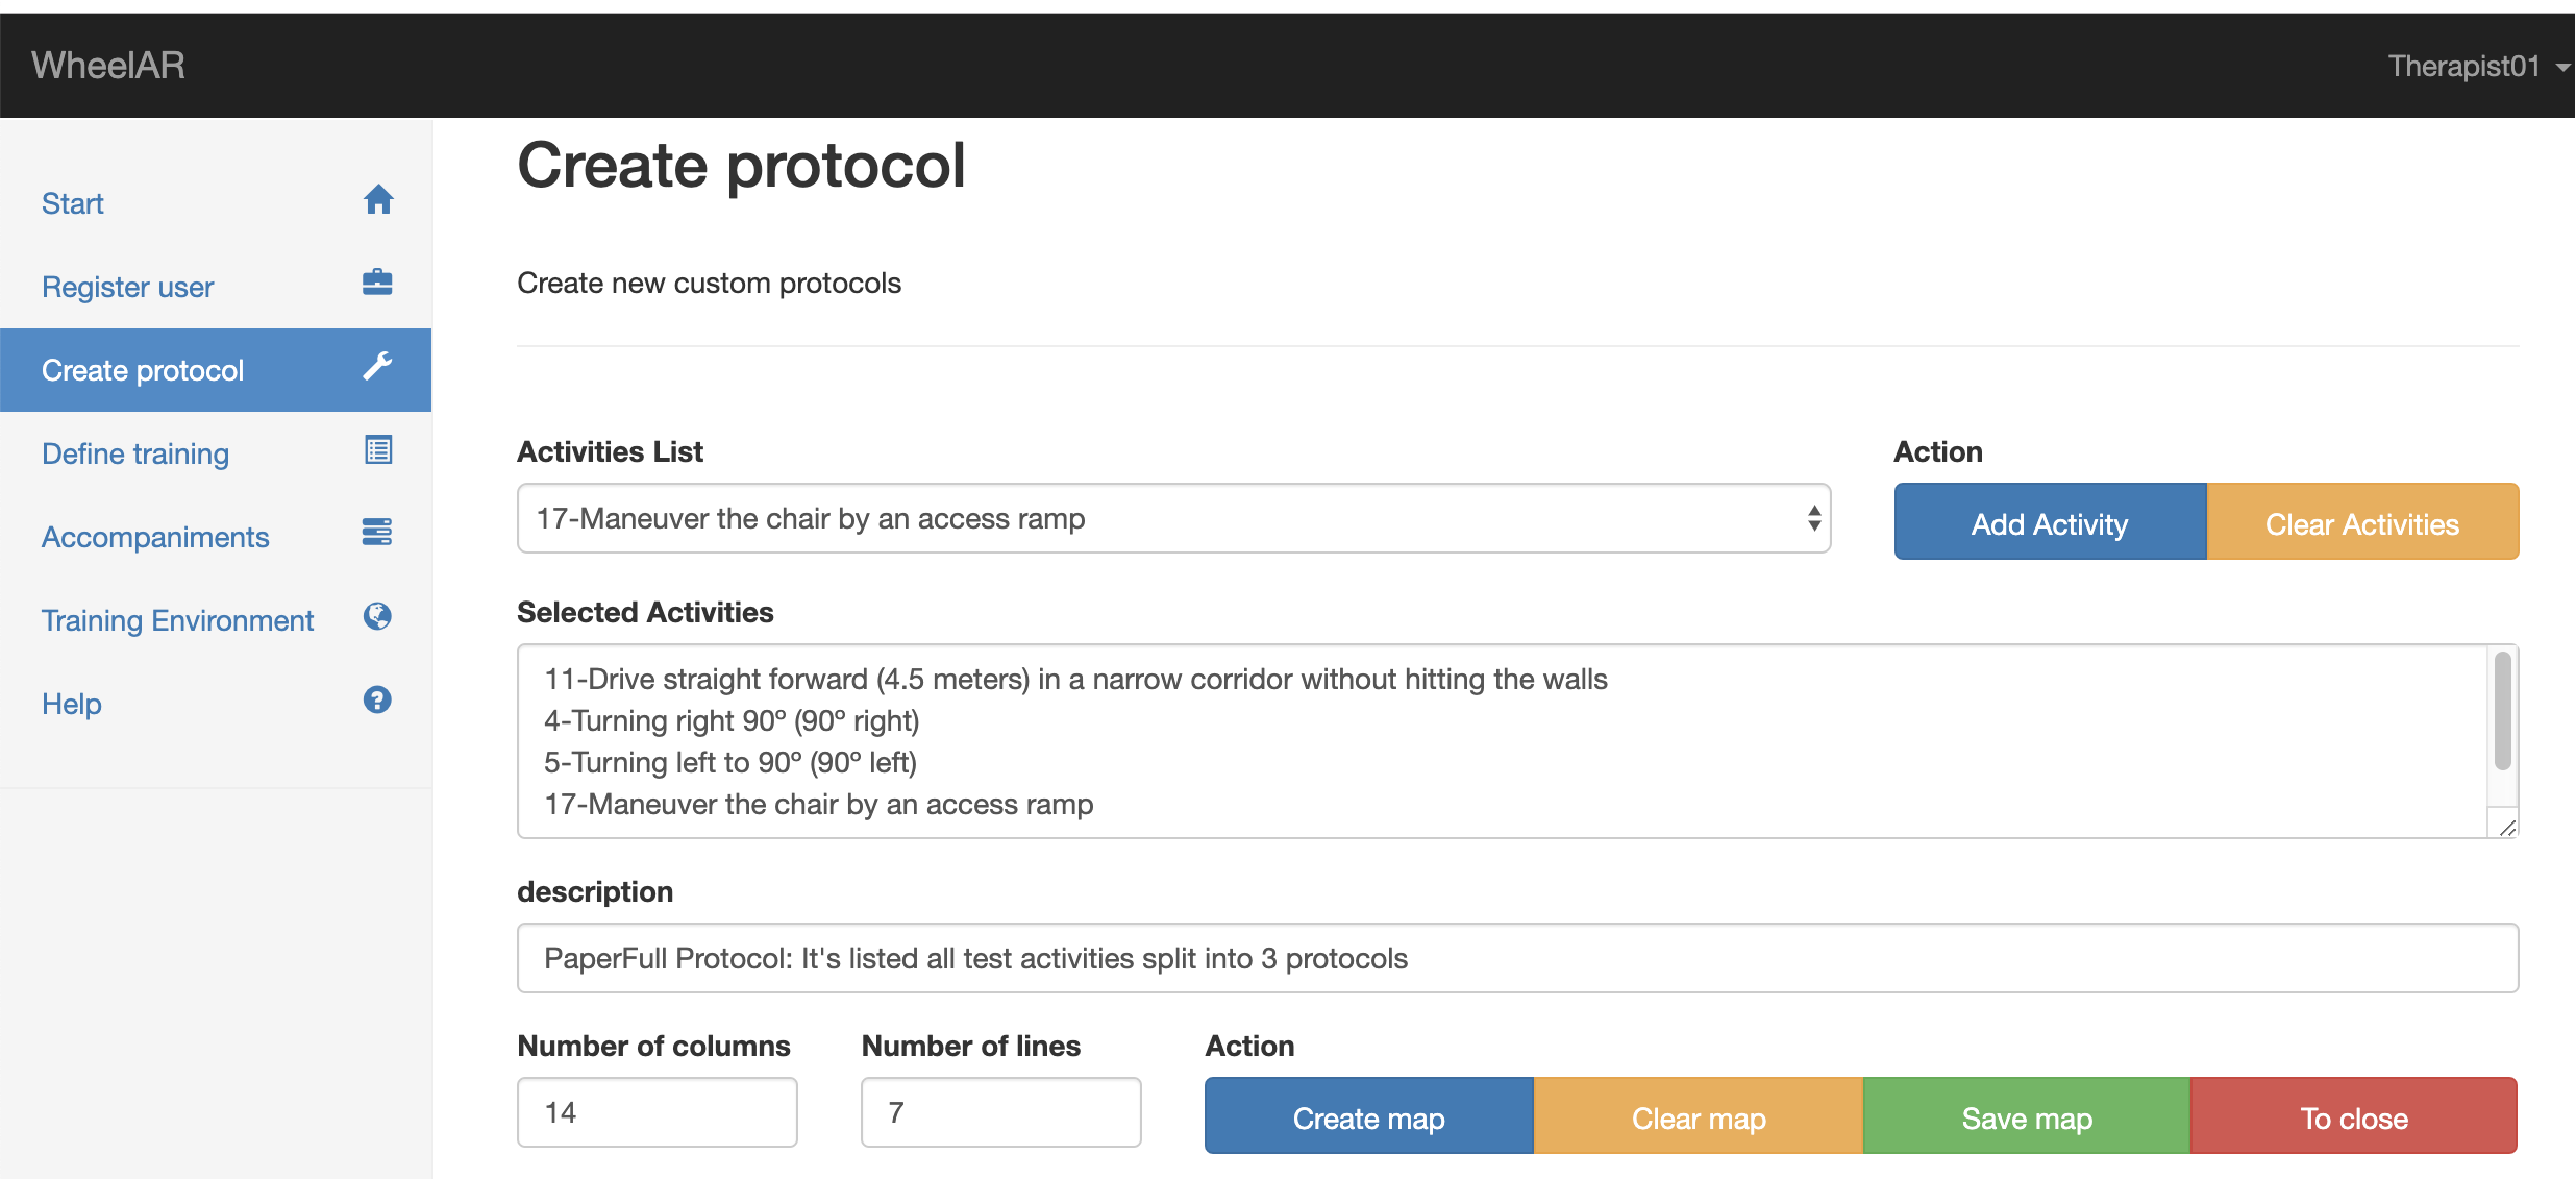
\includegraphics[width=0.95\linewidth]{img/apendiceD/tCreateProtocol01}
\caption{Defining the activities for each protocol} \label{fig:apDcreateProtocol01}
\end{center}
\end{figure}

Next step is to fill a short description and next, to create the map of fiducial markers that's customise the training protocol. To use the whole area is necessary to set 14 columns and 7 lines number and  then click on ``Create map'' to create an empty map or click on ``Clear map'' to remove the created map.
The fiducial AR matrix is initially filled with numbered indexed buttons which means that no virtual object was attached yet. All red buttons presented in Figure \ref{fig:apDcreateProtocol02}  have physical equipments that can be used by the therapist on training protocol.  

\begin{figure}[!hbt]
\begin{center}
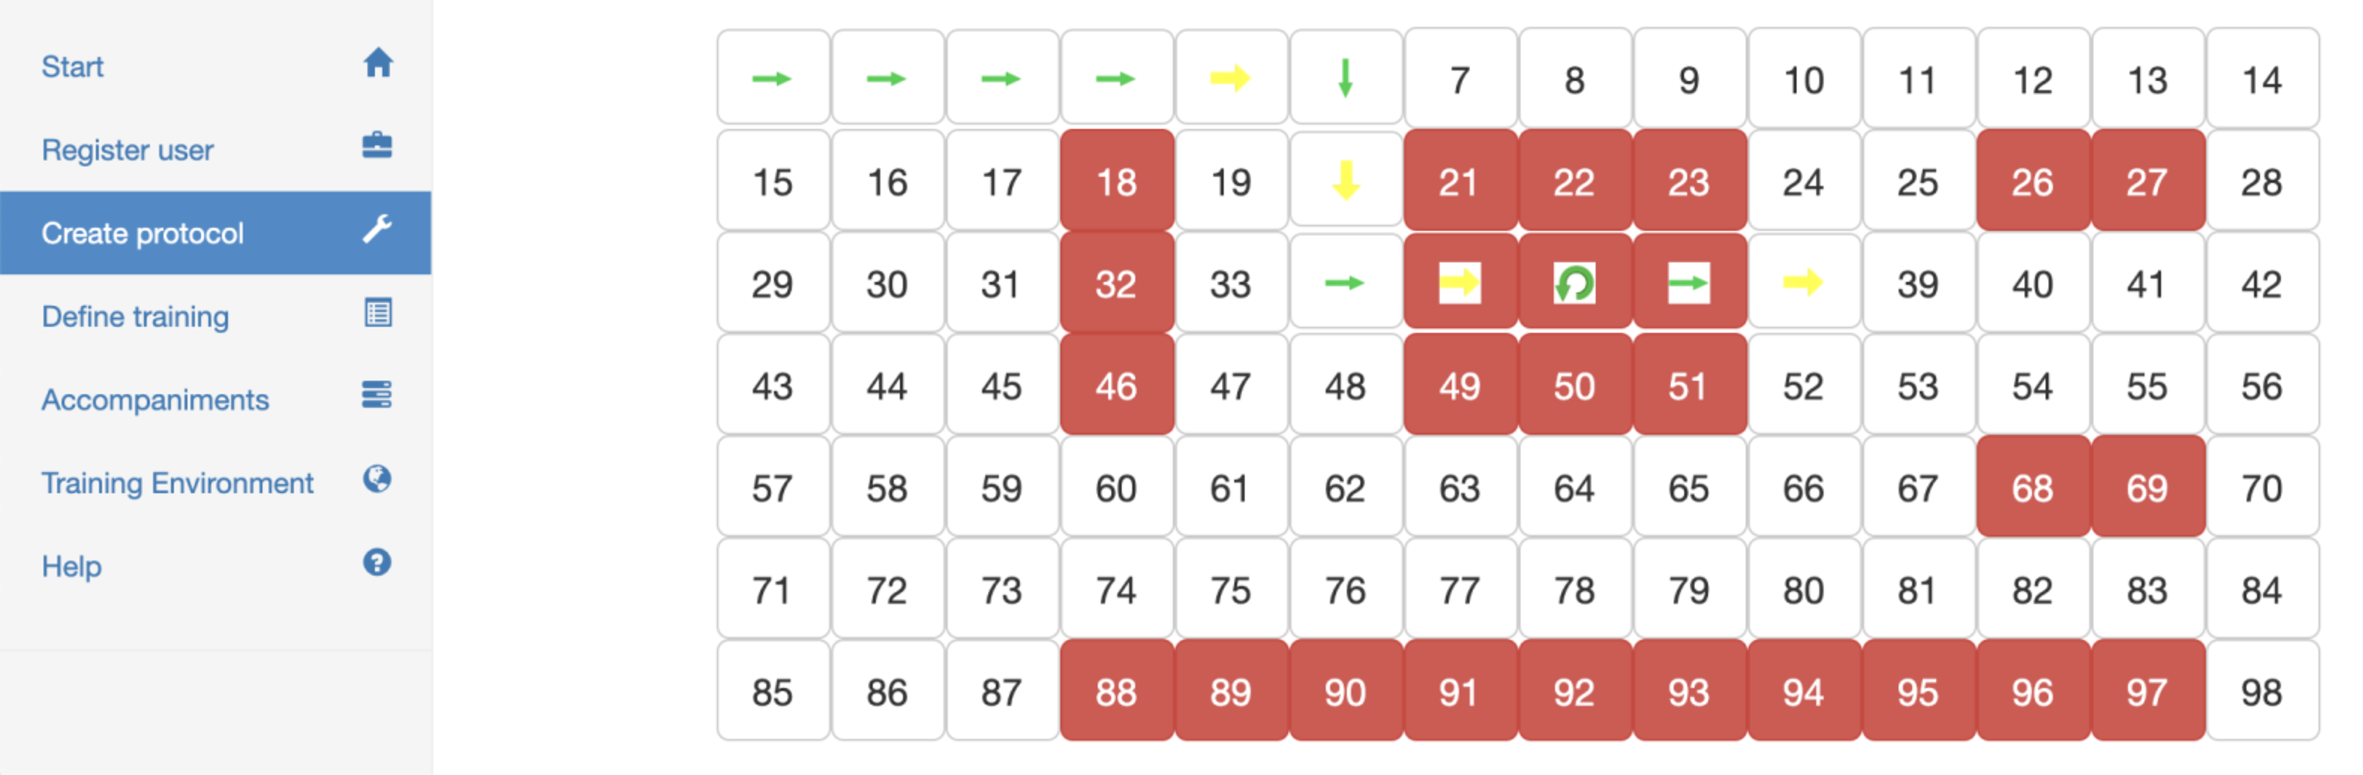
\includegraphics[width=1\linewidth]{img/apendiceD/tCreateProtocol02}
\caption{Create a training activities and protocol map example} \label{fig:apDcreateProtocol02}
\end{center}
\vspace{-15pt}
\end{figure}

Virtual object that can be used as a guidance or avoidance and also can be static or animated. Thus, is possible even in a controlled environment have non-structural activity in where the user have to decide what he have to do in front of an unexpected event. To insert a virtual object it is necessary to click in each marker and then select one of the objects presented in Figure \ref{fig:apDvirtualObjects}. Green arrows is used as a guidance and the yellows arrows means the end of an activity proposed by the therapist. 

\begin{figure}[!hbt]
\begin{center}
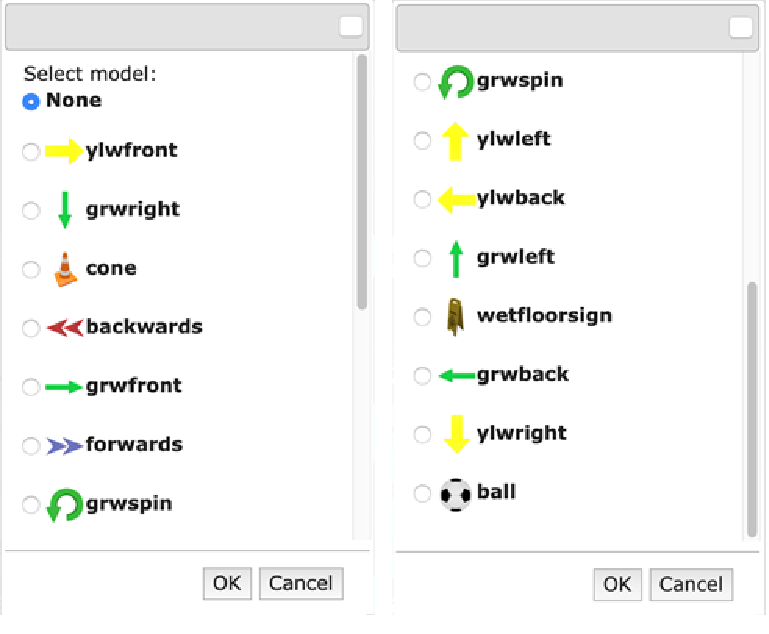
\includegraphics[width=0.5\linewidth]{img/apendiceD/virtualObjects}
\caption{Virtual objects (animated/statics) list} \label{fig:apDvirtualObjects}
\end{center}
\vspace{-15pt}
\end{figure}

Figure \ref{fig:apDcreateProtocol02} is a protocol example. Protocols can be saved clicking on ``Save map'' or to exit to the system ``To close''. 

\subsubsection{Define protocol}
\label{sec:appDefineProcotol}

In this section page, the therapist preview all training sessions requested from different user's. From ``Select the protocol'', the therapist is able to choose all training protocol created from him and preview some informations about it, as presented from Figure \ref{fig:apDtDefineProtocol01} and also, to visualise the ``Training Environment'' is \textbf{Free} or \textbf{Occupied}.

\begin{figure}[!hbt]
\begin{center}
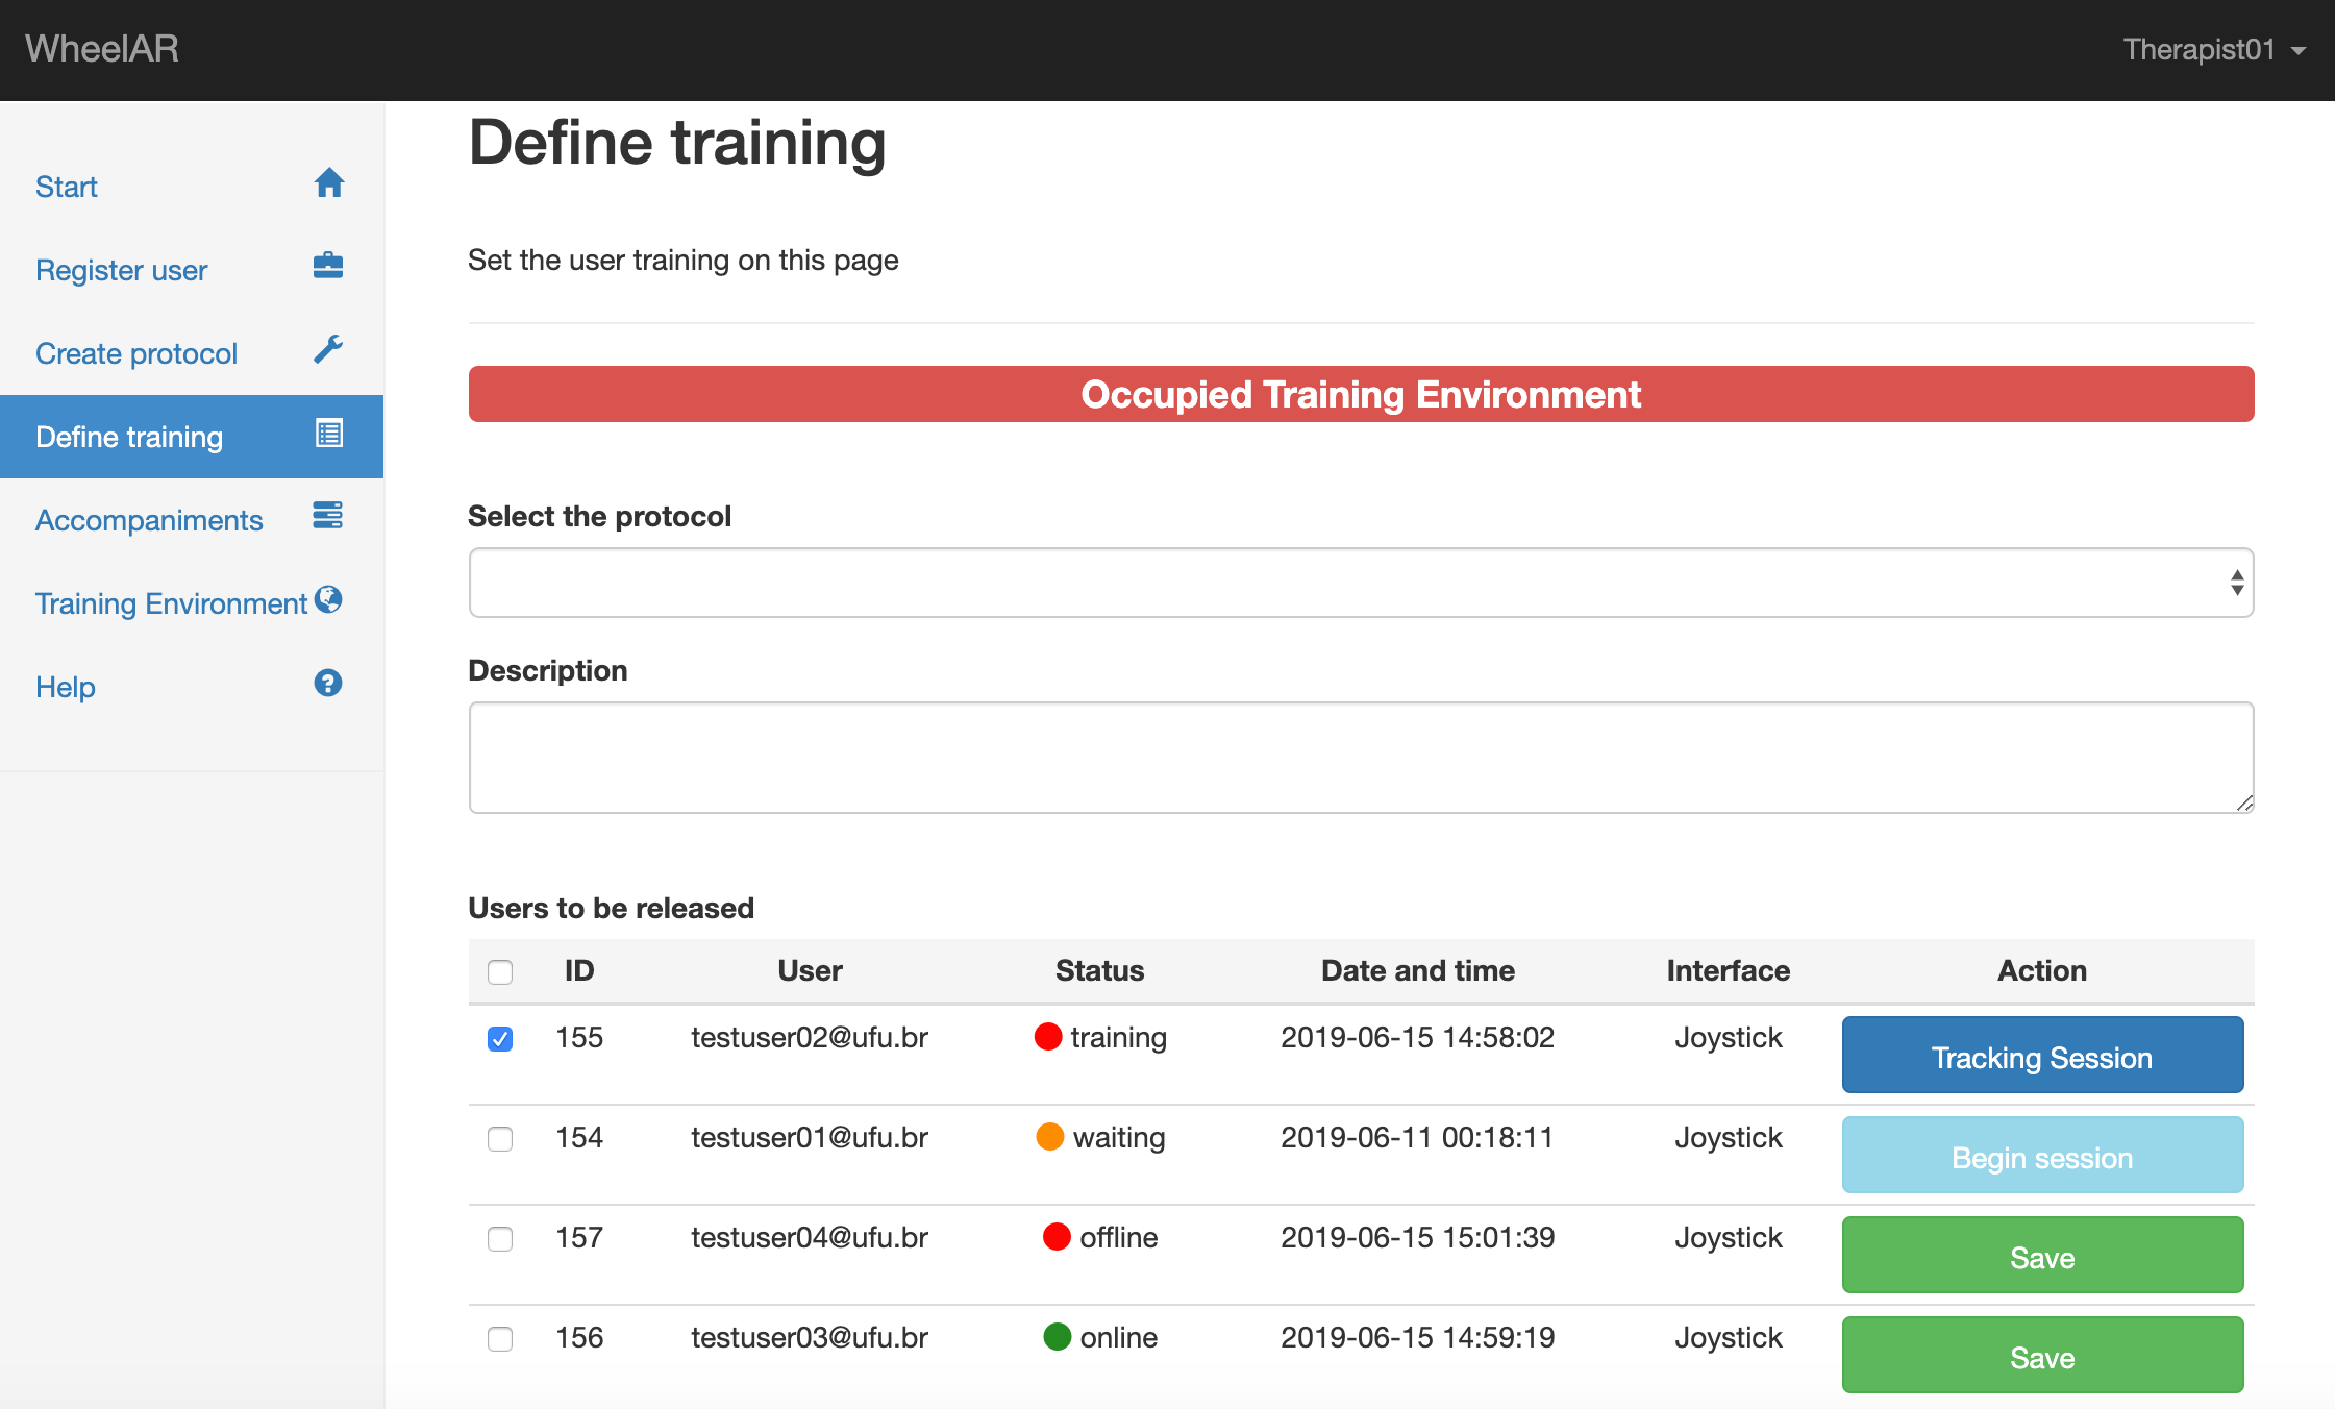
\includegraphics[width=1\linewidth]{img/apendiceD/tDefineProtocol01}
\caption{Define training protocol} \label{fig:apDtDefineProtocol01}
\end{center}
\vspace{-15pt}
\end{figure}

Before selecting one of the existents actions: ``Save'', ``Begin session'' and ``Tracking session'' is  necessary to be aware of  each users status means, as presented by Figure \ref{fig:apDtDefineProtocol01}:

\begin{enumerate}
\item \textit{Status}:
\begin{enumerate}[label=(\alph*)]
\item \textbf{Offline}: The user may have already requested a training, but is not connected into the system;
\item \textbf{Online}: The user may have already requested a training, but is not waiting for the release. After a request is made, the system will only include a new one after the last request is made;
\item \textbf{Waiting}: After clicking on the connect button, as shown in Figure \ref{fig:apDtUserSession}, the user should wait for the therapist to release the training;
\item \textbf{Training}: Defined the training protocol, released and initialized video streaming, the control commands are forwarded allowing the user to execute the protocol defined by the therapist. The environment is locked during this time.
\end{enumerate} 
\item \textit{Actions}: The actions below have to execute following the order.
\begin{enumerate}[label=(\alph*)]
\item \textbf{Save}: Check the training request and press the button. Now, the therapist is able to perform the next action;
\item \textbf{Begin session}: All training requisition who have a training protocol defined can be started while the training environment is free. Them, press the button to be redirected to ``Start streaming page'' action was mentioned before in Section \ref{sec:impltrainingsite}. 
\item \textbf{Tracking session}: Soon as the training is released by pressing this button the therapist is redirected to the ``Waiting pages'' and then to the ``Therapist Viewport page'' presented in Figure \ref{fig:apDtViewPortTherapist}. Now, he can follow the user training and interact with the PW. Throughout the session, the therapist has to press the ``Mark activity'' button when the user passes over a yellow marker,  to counts commands entered and also the time spent during the activity. Finished the training by the user,  the ``Close tracking'' has to be pressed to be redirected to the next action.
\end{enumerate} 
\end{enumerate}

\begin{figure}[!hbt]
\begin{center}
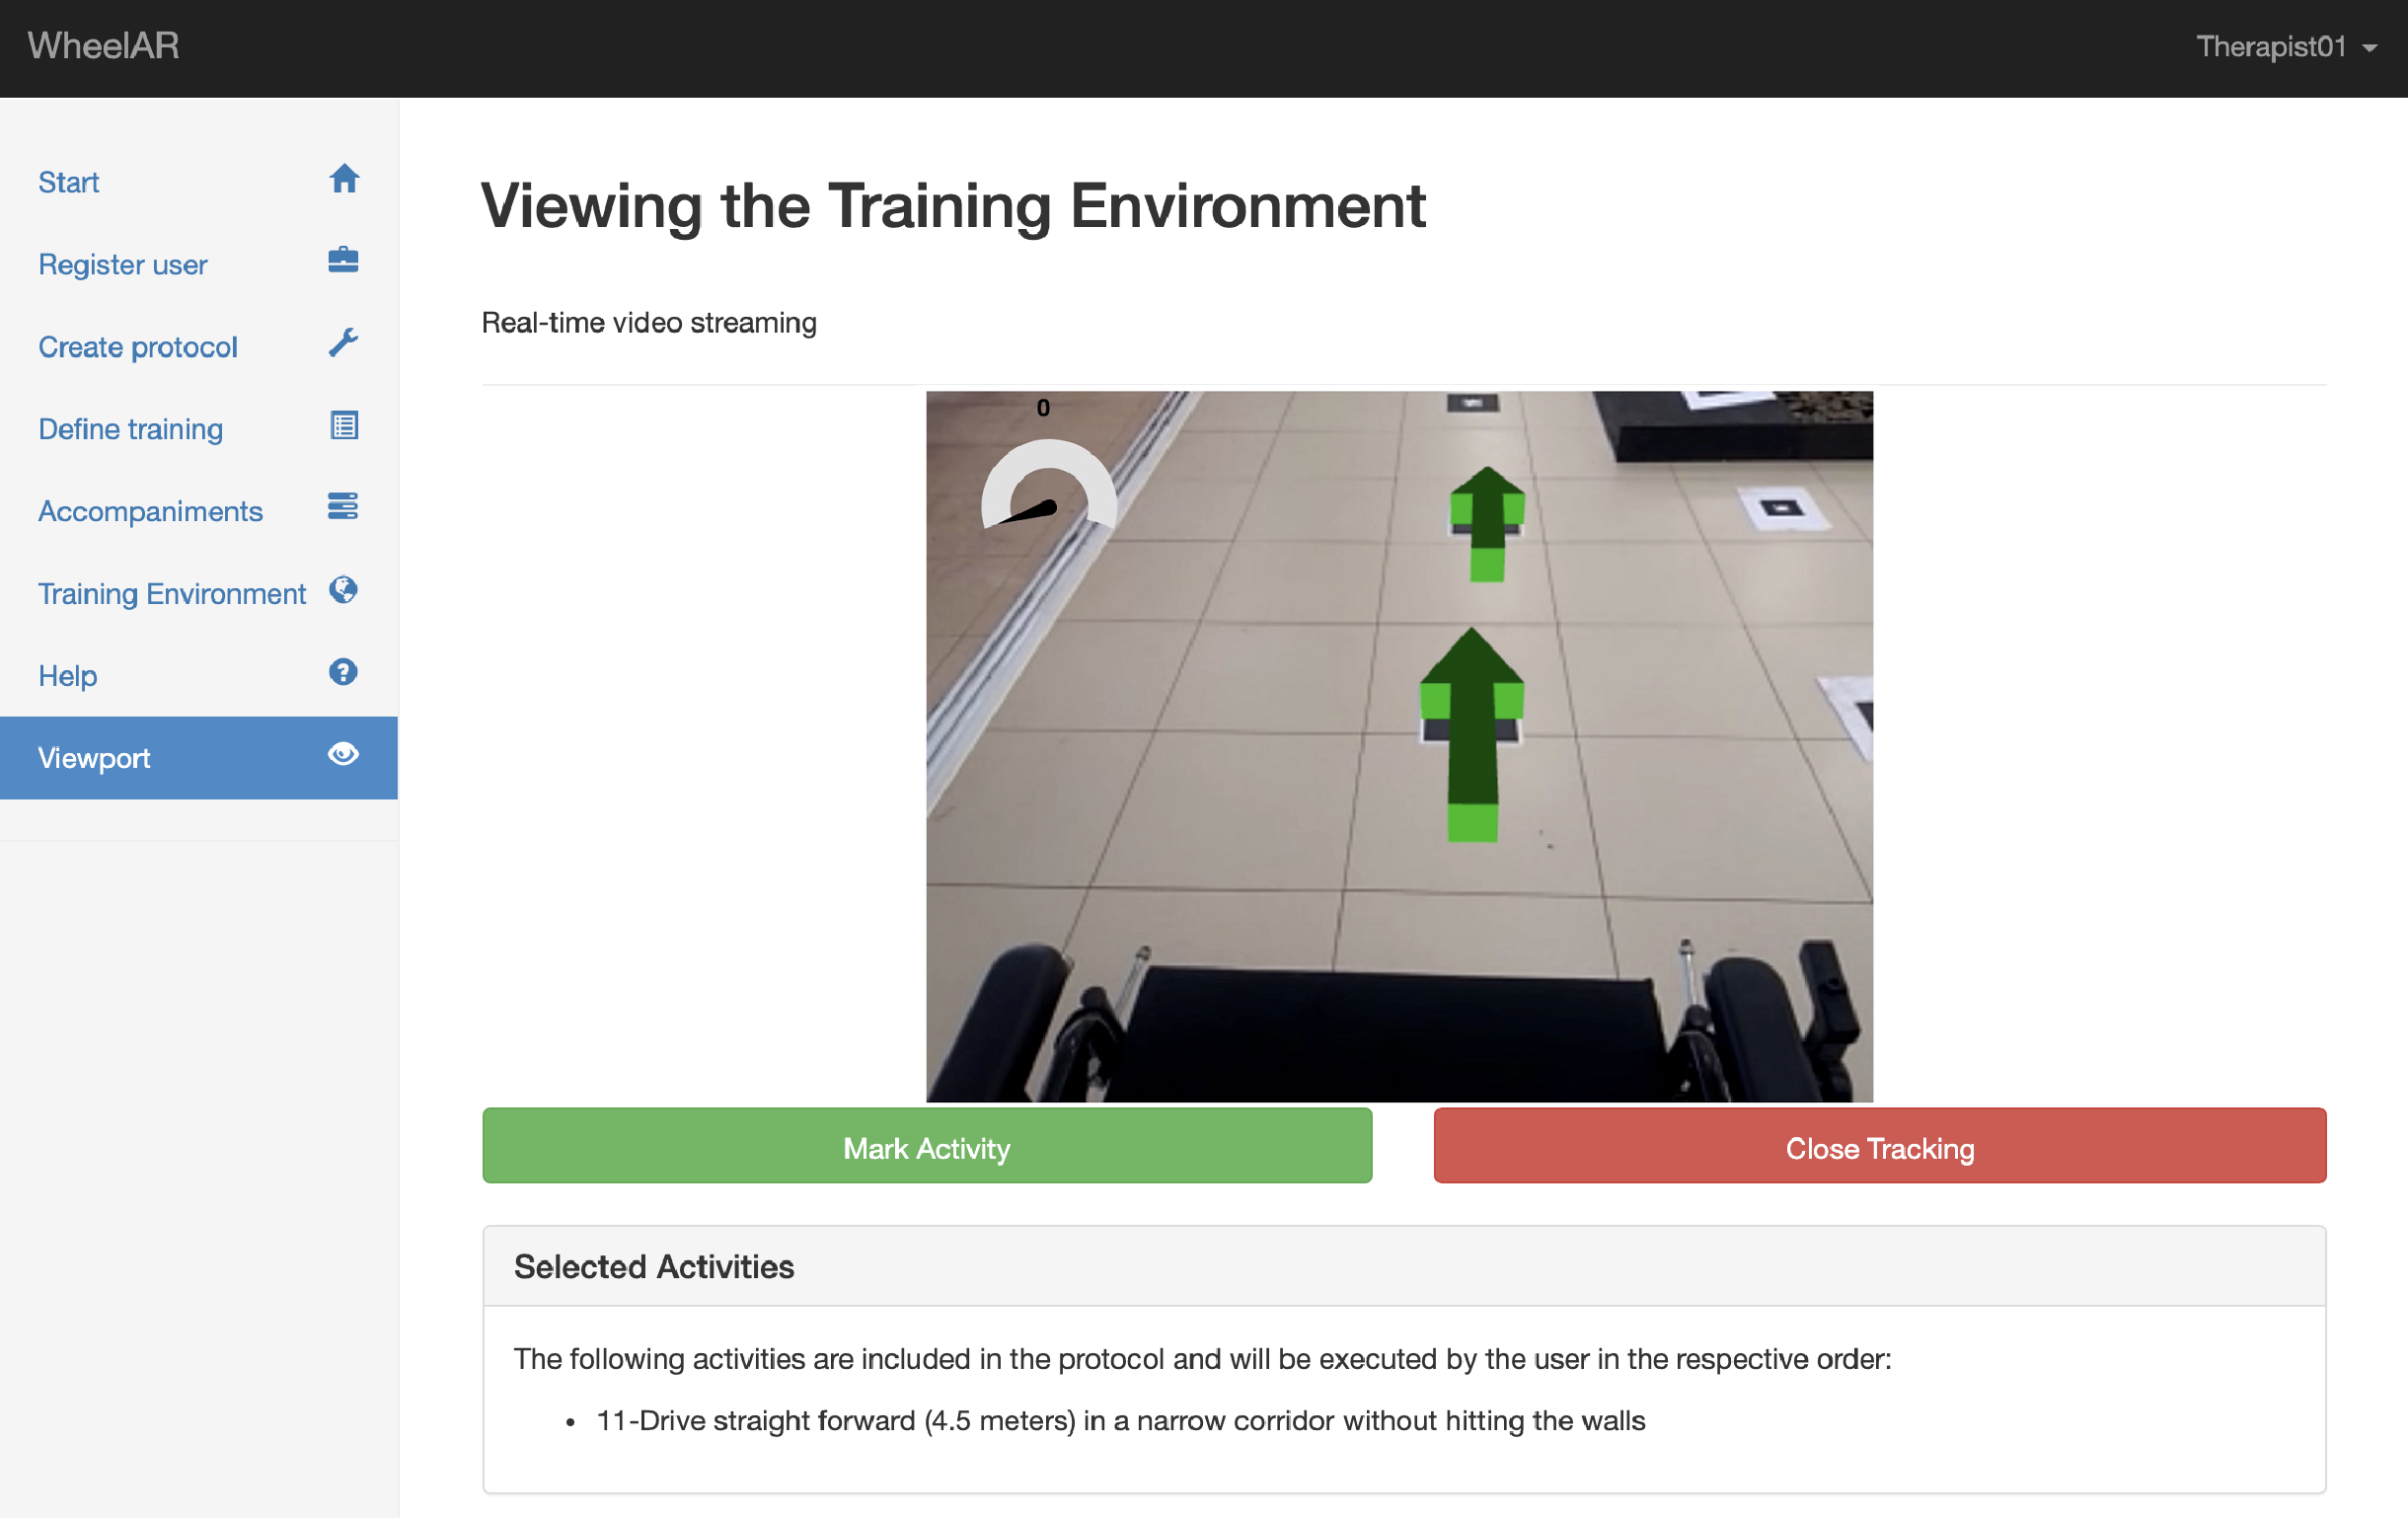
\includegraphics[width=1\linewidth]{img/apendiceD/tViewPortTherapist}
\caption{Tracking session and Therapist ViewPort page} \label{fig:apDtViewPortTherapist}
\end{center}
\end{figure}


\subsubsection{Evaluate training}

Based on PMRT Assessment Form, the system retrieves all information stored into the database of each activity. The therapist only have to fill out the comments around, collision number and then choose a relative note. Before saving the evaluation, the ``Calculate score'' button is triggered to update the score. Thus, the system redirects to the therapist ``Annotations page''.  

\begin{figure}[!hbt]
\begin{center}
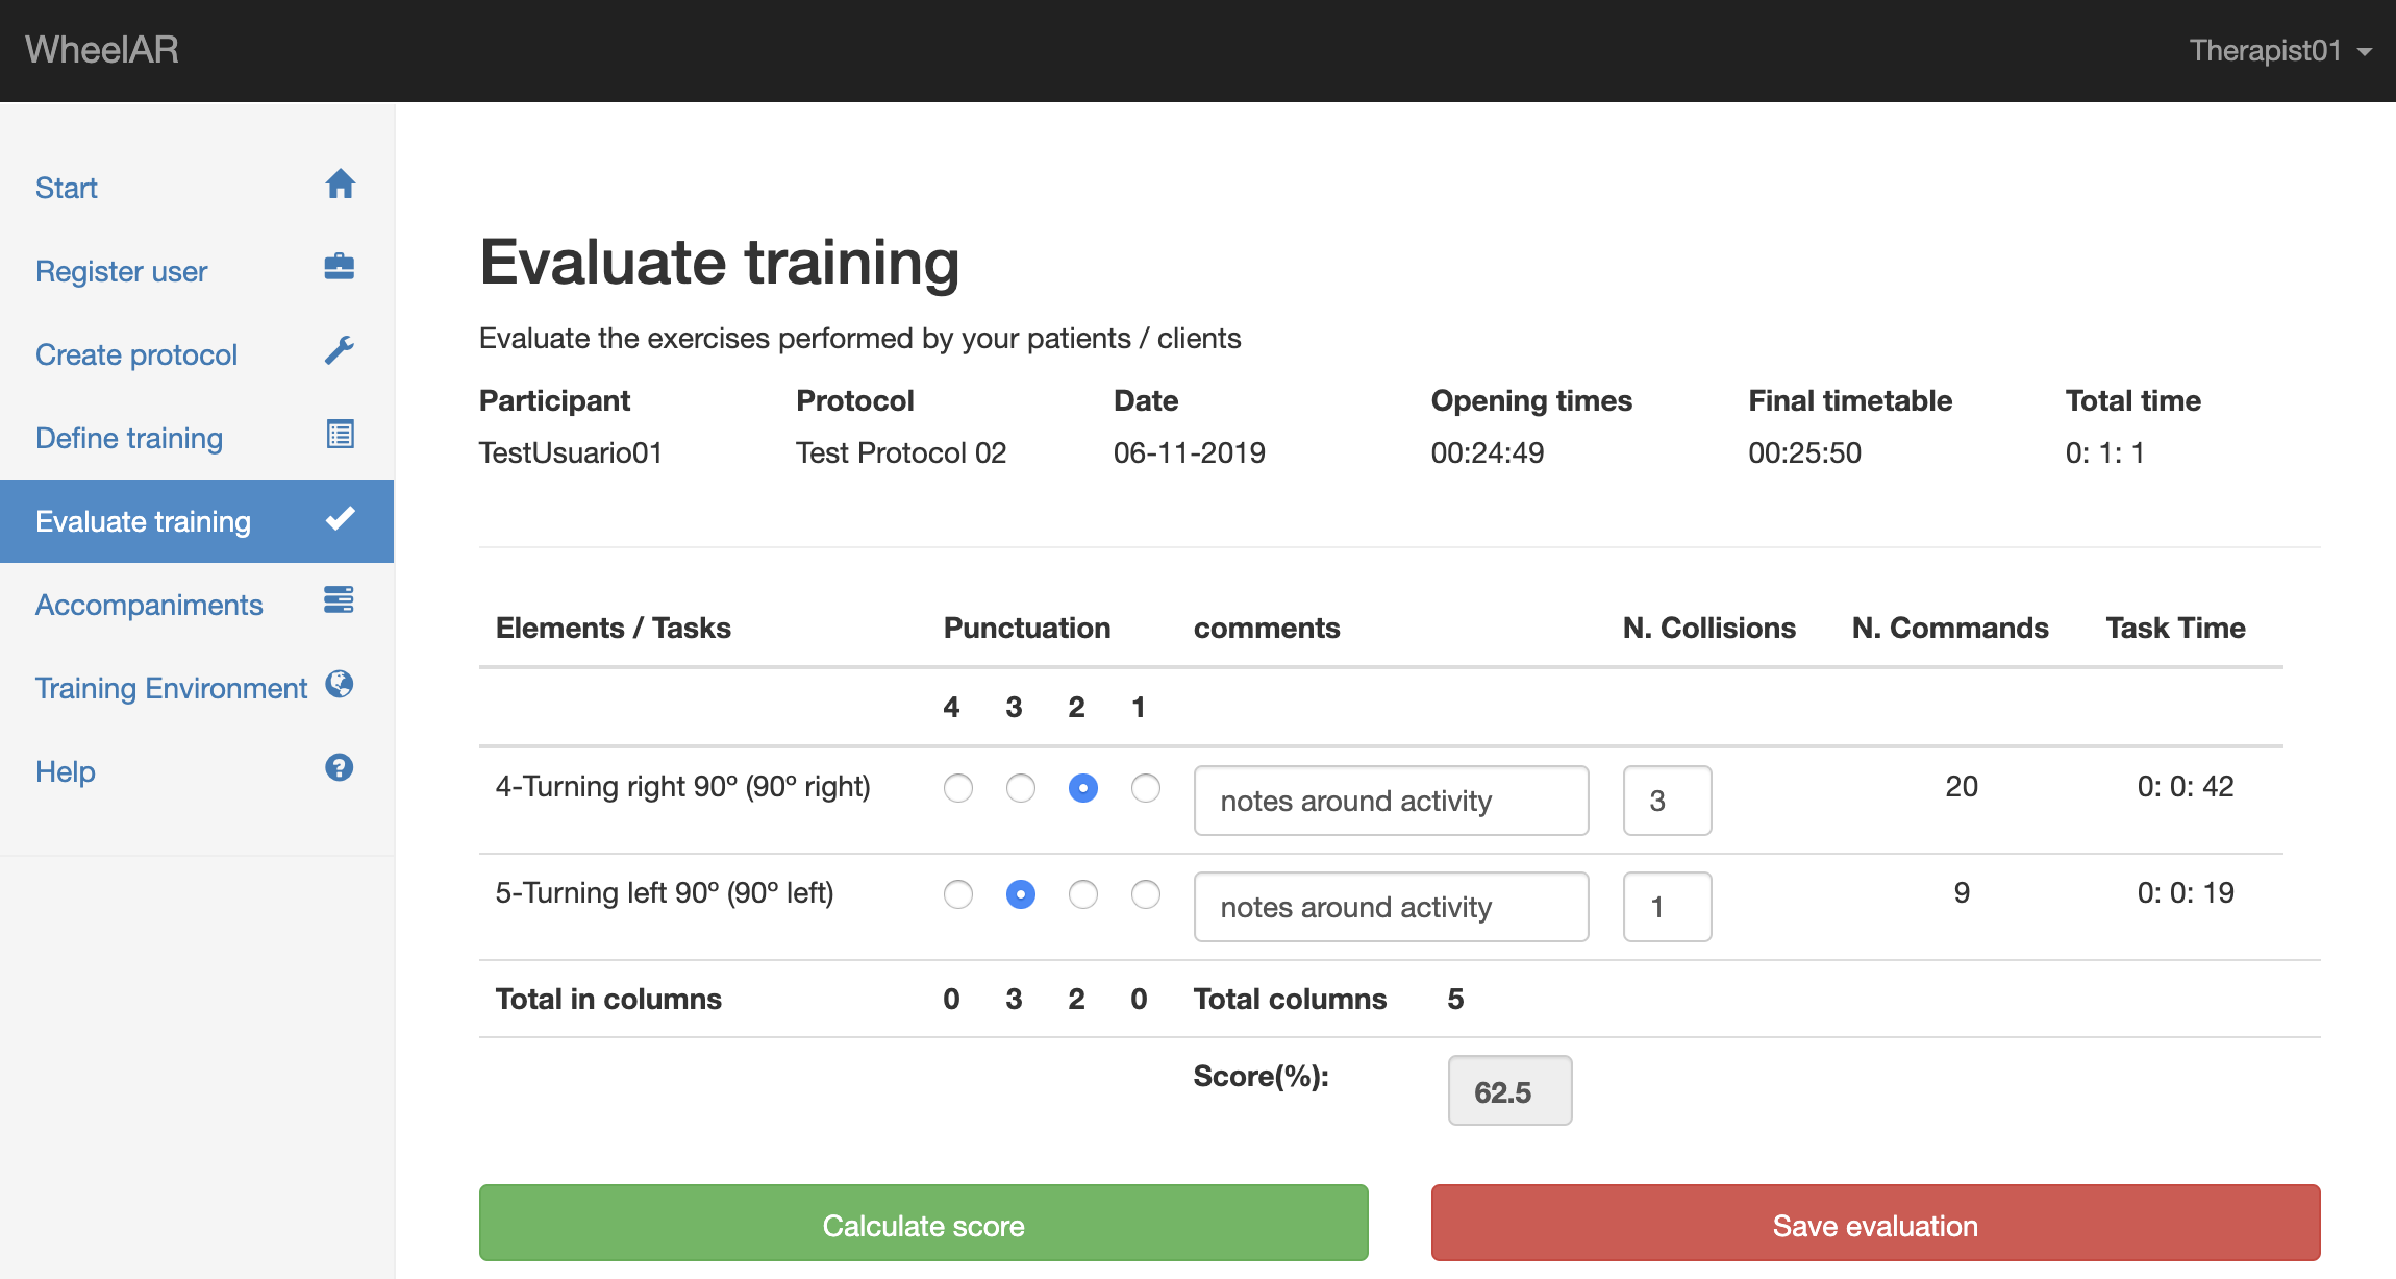
\includegraphics[width=1\linewidth]{img/apendiceD/tEvaluateTraining}
\caption{Adapted PMRT Evaluation Form} \label{fig:apDtEvaluateTraining}
\end{center}
\vspace{-15pt}
\end{figure}


\subsubsection{Annotations}

In this page, the therapist is able to take some general or complementary notes information about the user evolution, during training sessions, to all activities into to training protocol, as shown in Figure \ref{fig:apDtAnnotations}. To end this task, the ``Save notes'' button is pressed saving the data into the ``historyTH'' database and finally redirected to ``Start page'' where to start any other action like ``Accompaniments''. 

\begin{figure}[!hbt]
\begin{center}
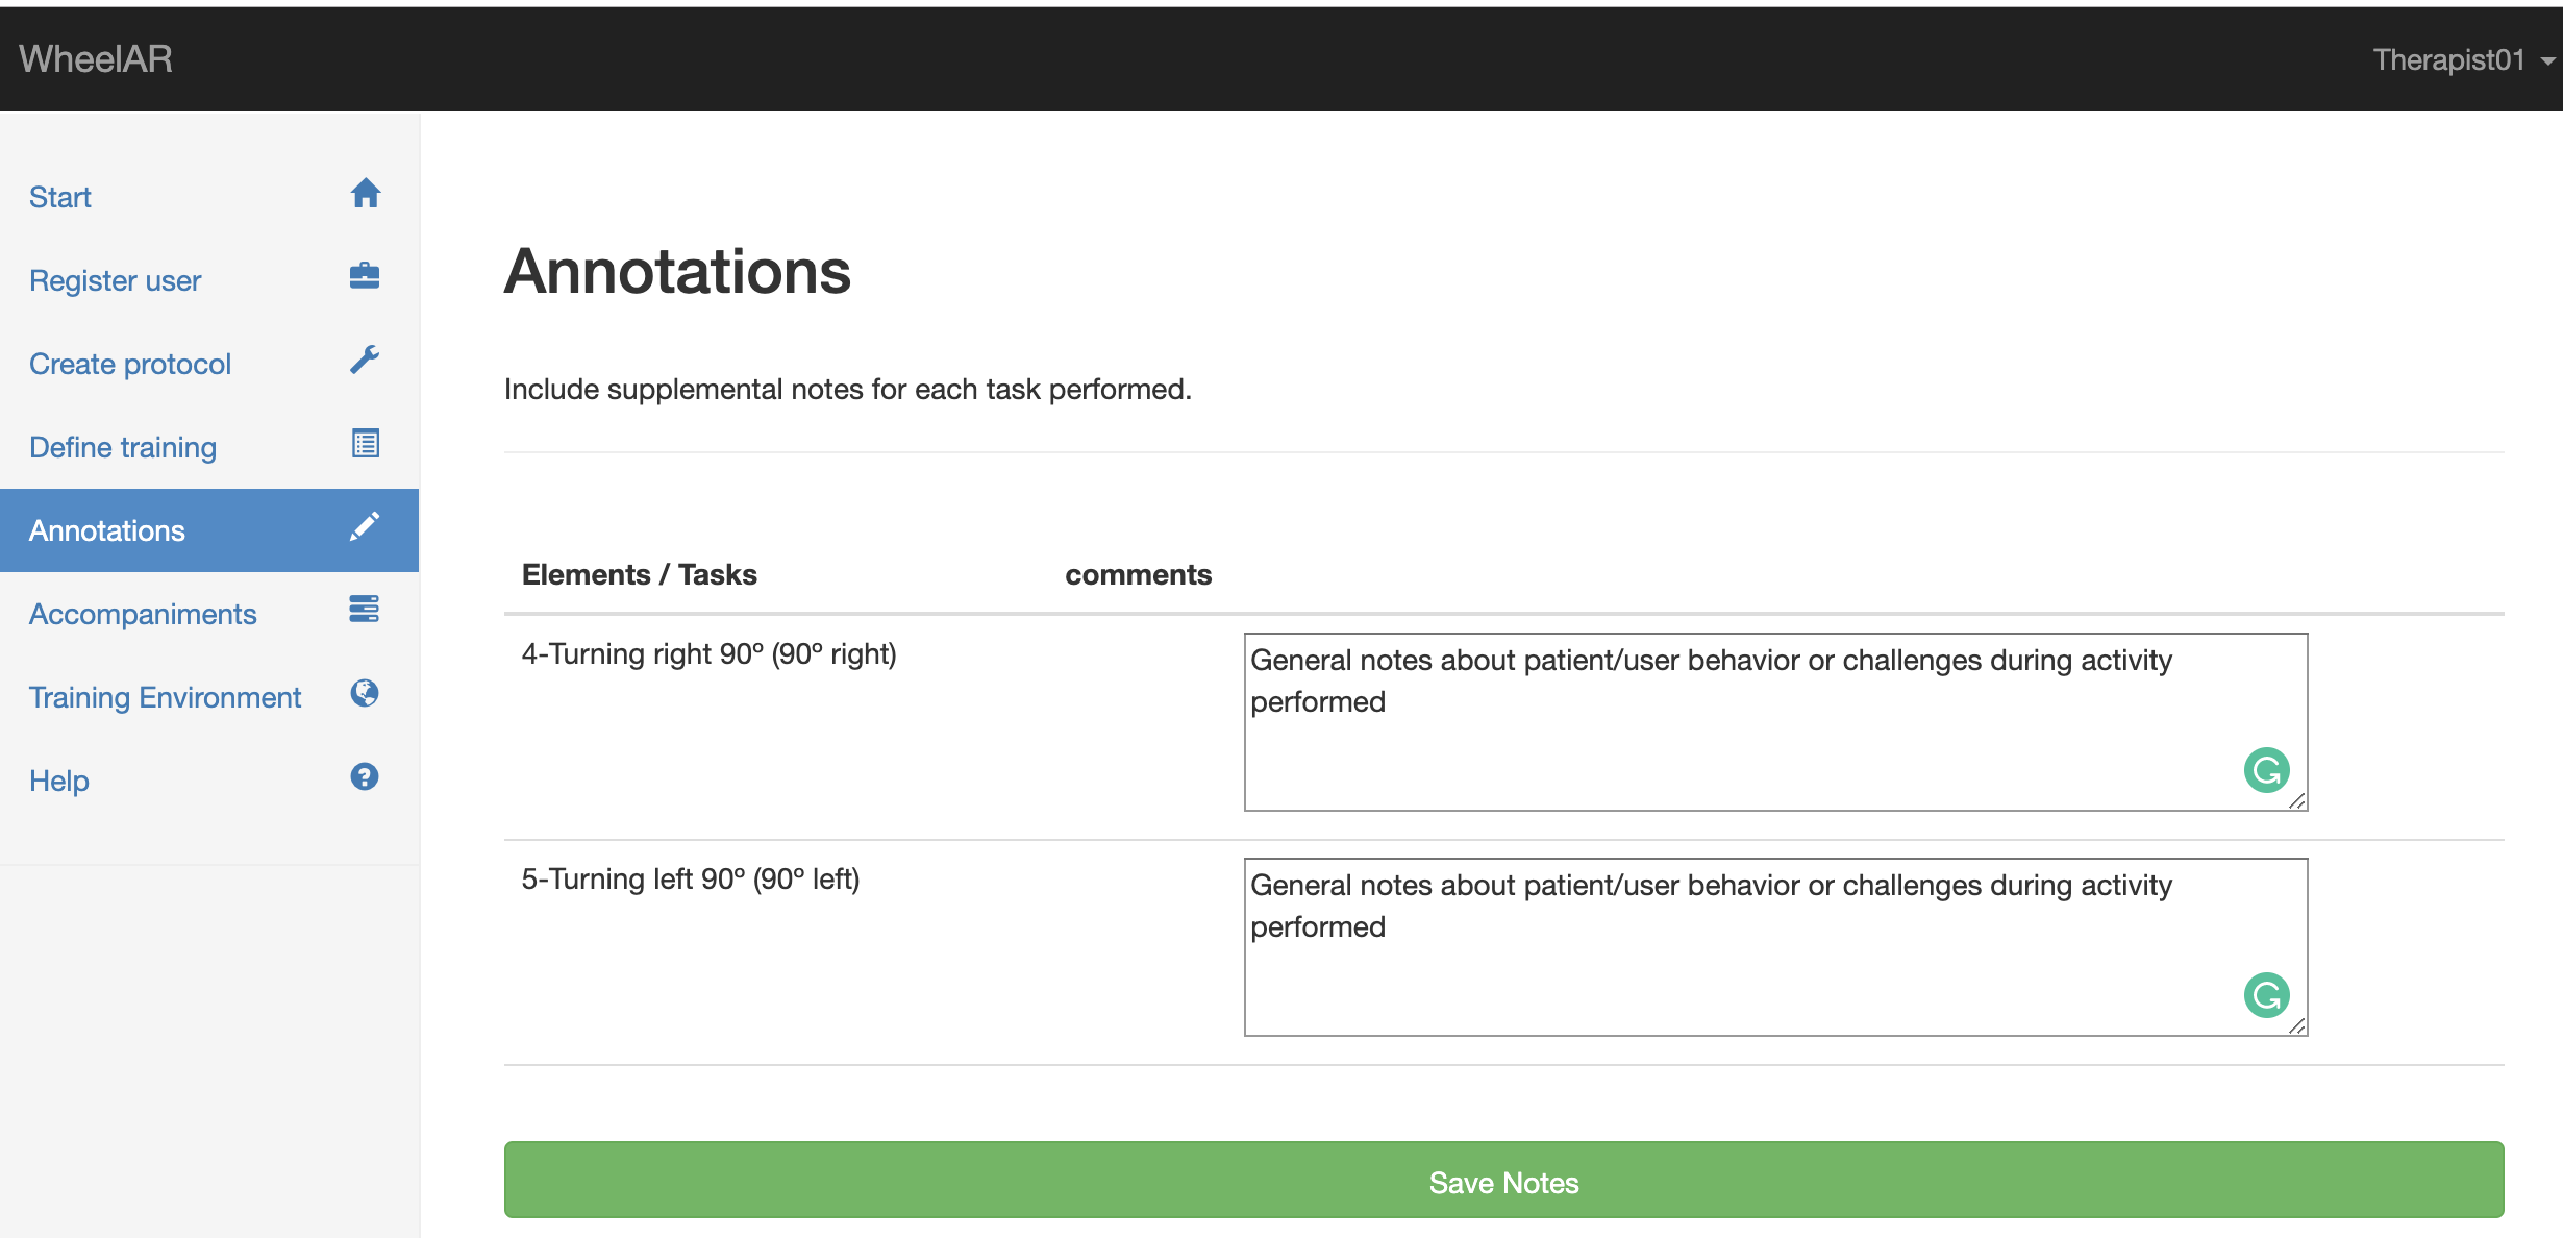
\includegraphics[width=1\linewidth]{img/apendiceD/tAnnotations}
\caption{General and clinicians notes around the user evolution} \label{fig:apDtAnnotations}
\end{center}
\vspace{-15pt}
\end{figure}

\subsubsection{Accompaniments}

Looking for clues of the user evolution after the training sessions, the therapist evaluates the graph presented by Figure \ref{fig:apDtGenerateChart02}. This graph can be generated in real-time and to do it, the following actions must be performed:

\begin{itemize}
\item \textbf{Select}: Select a patient from the ``Select patient'' list and click on the ``Select''  button to retrieve the files executed by the patient without a database. 
\item \textbf{Generate graph}: Afterwards, select one of the files in the ``Select the protocol'' list and click the ``Generate graph'' button. 
\end{itemize}

On the y-axis, there are quantitative information regarding a number of commands, collisions, time spent and note reached, as shown in the chart legend. On the x-axis, the protocols are separated into sets by ID and Data. The activities in each are grouped, allowing a different analysis.

\begin{figure}[!hbt]
\begin{center}
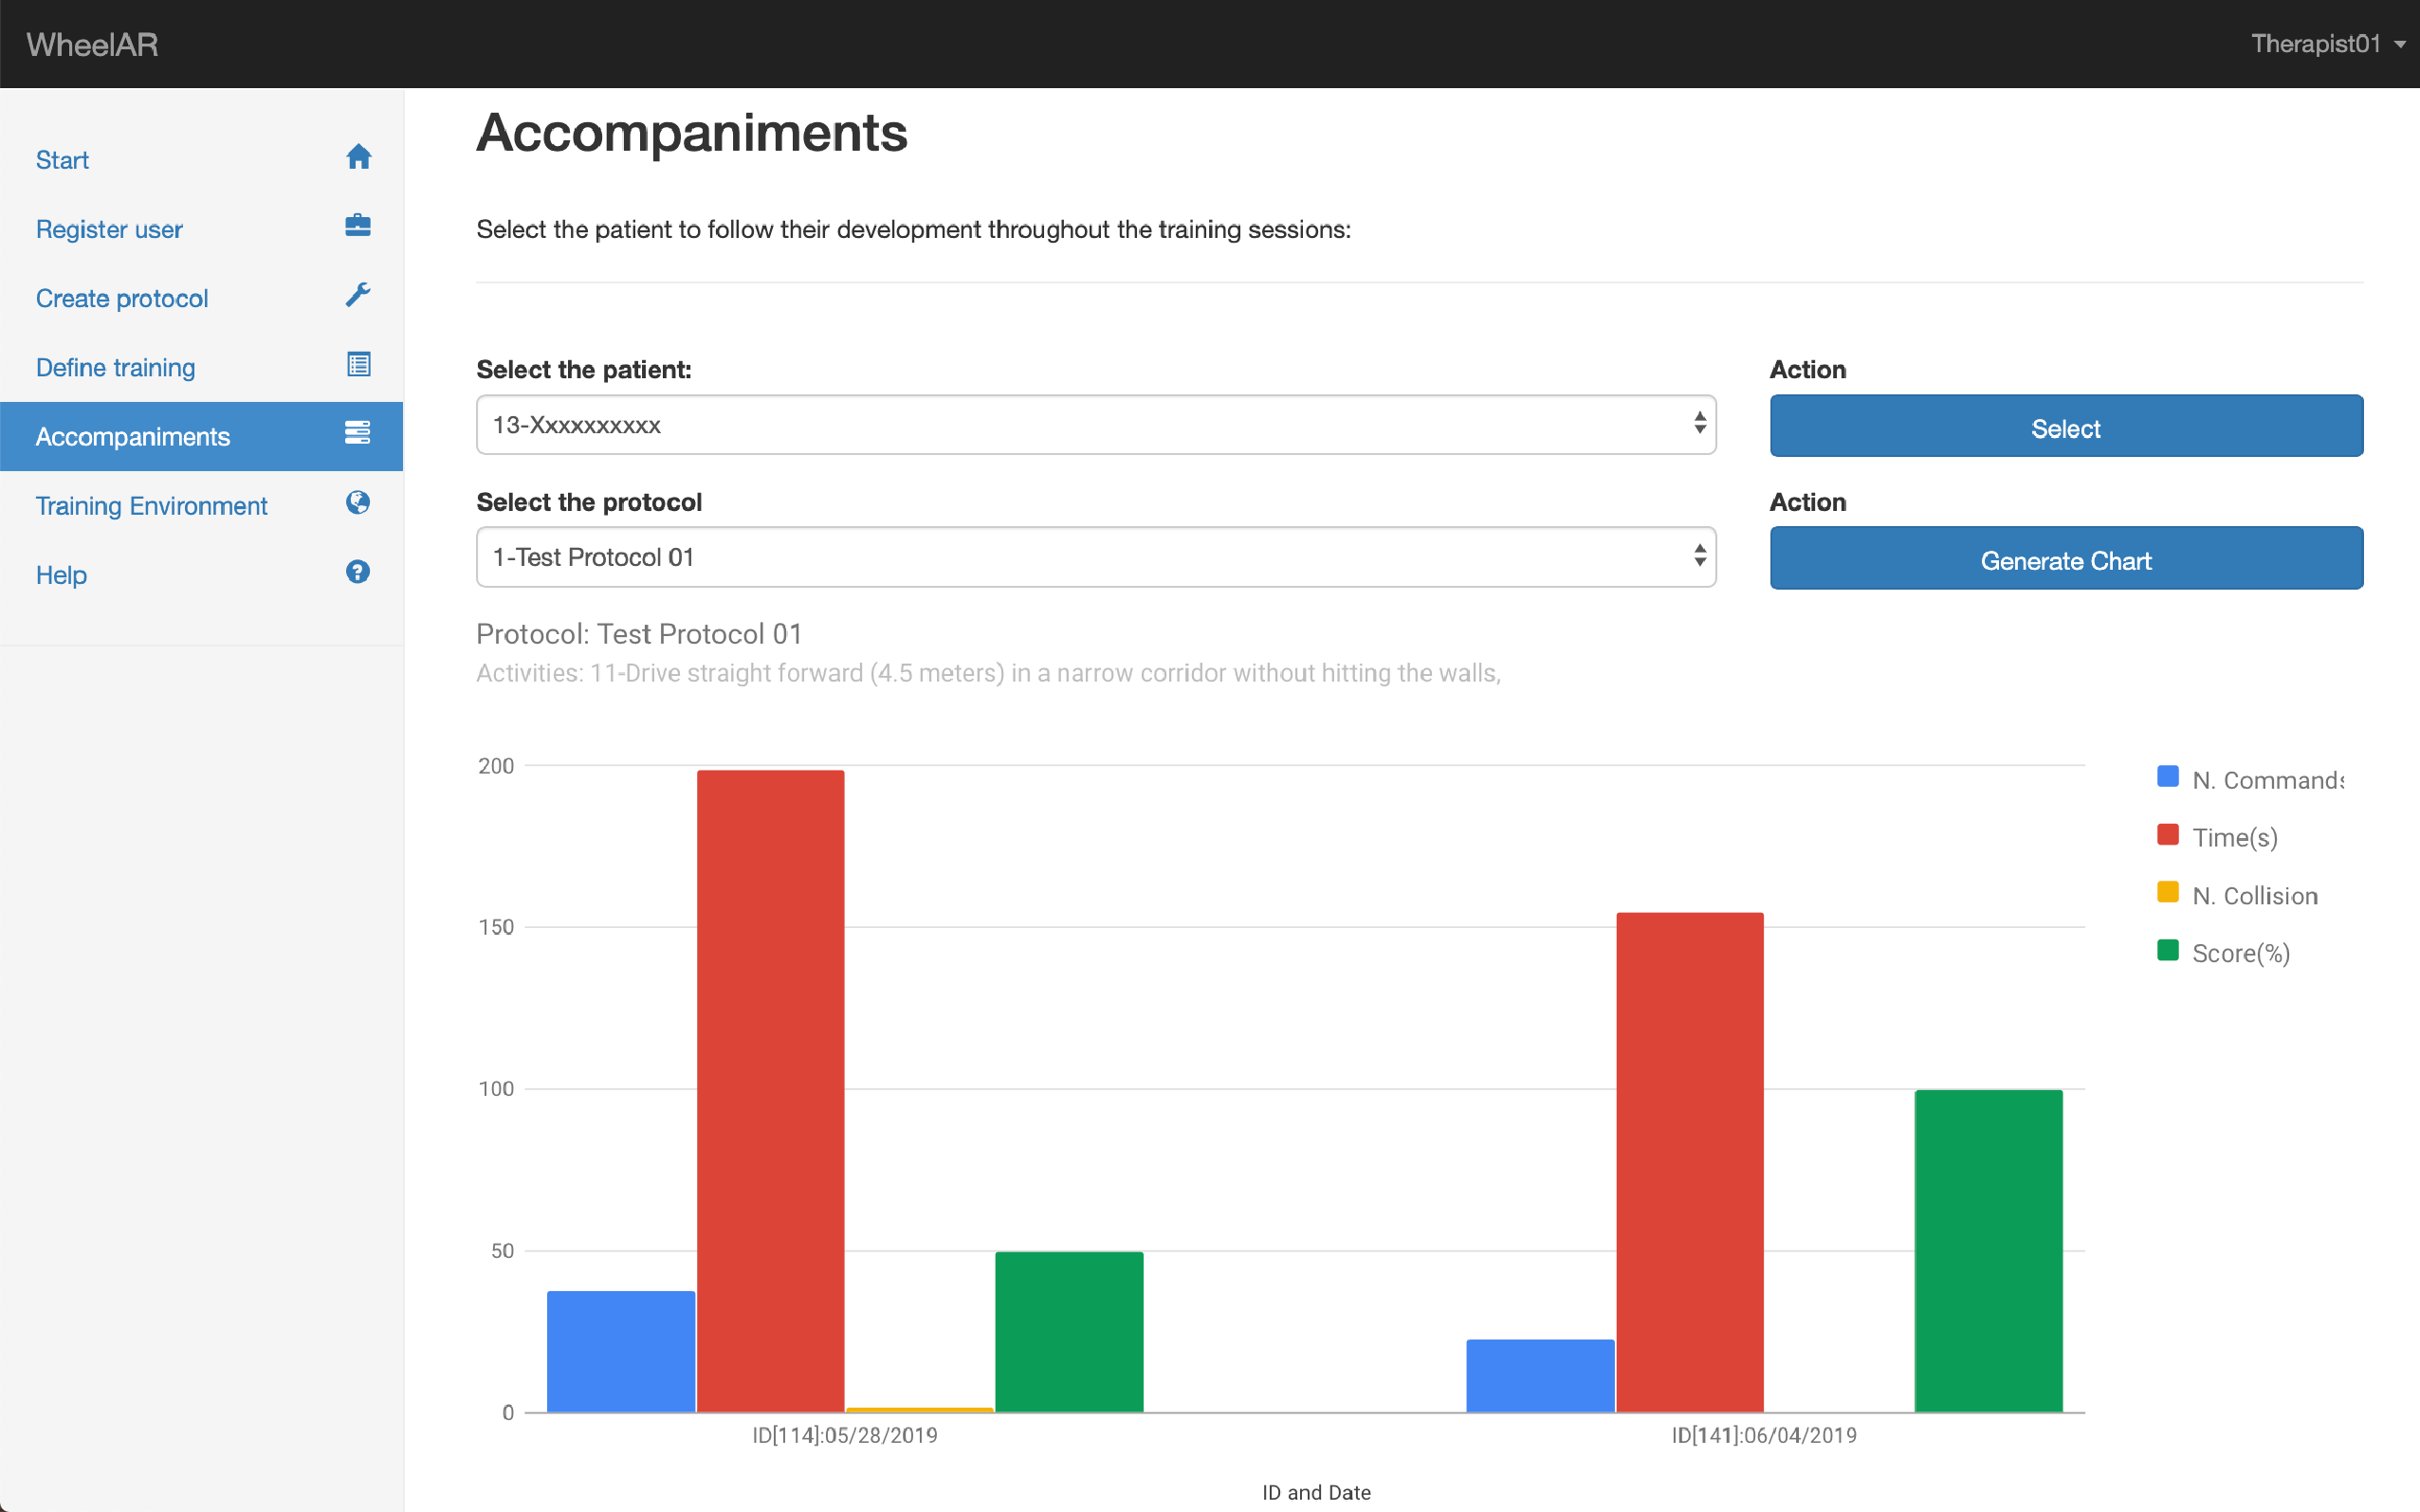
\includegraphics[width=1\linewidth]{img/apendiceD/tGenerateChart02}
\caption{Comparative chart users training protocols performed} \label{fig:apDtGenerateChart02}
\end{center}
\vspace{-15pt}
\end{figure}


In addition to this graph, information about the SI or excitation from the biosignals allows the evaluation of the emotional state of the same, helping also in the understanding of the real difficulties and observing the overcoming of them after each session. 


\subsection{User session}

Once the user has logged into the system, his status is updated to ``on-line'', which means that he is connected but not in training process. After, the user is invited to select an interface control existent such as a keyboard, joystick, and others and then press the button ``Connect'' to request a new training session, as presented in Figure \ref{fig:apDtUserSession}. A new blank record is inserted on ``assessTH'' table responsible to store all data from training session changing the user status from ``on-line'' to ``waiting''. Otherwise, the user can press the button ``Close'' to  exit the system changing, his status to ``off-line''. 

\begin{figure}[!hbt]
\begin{center}
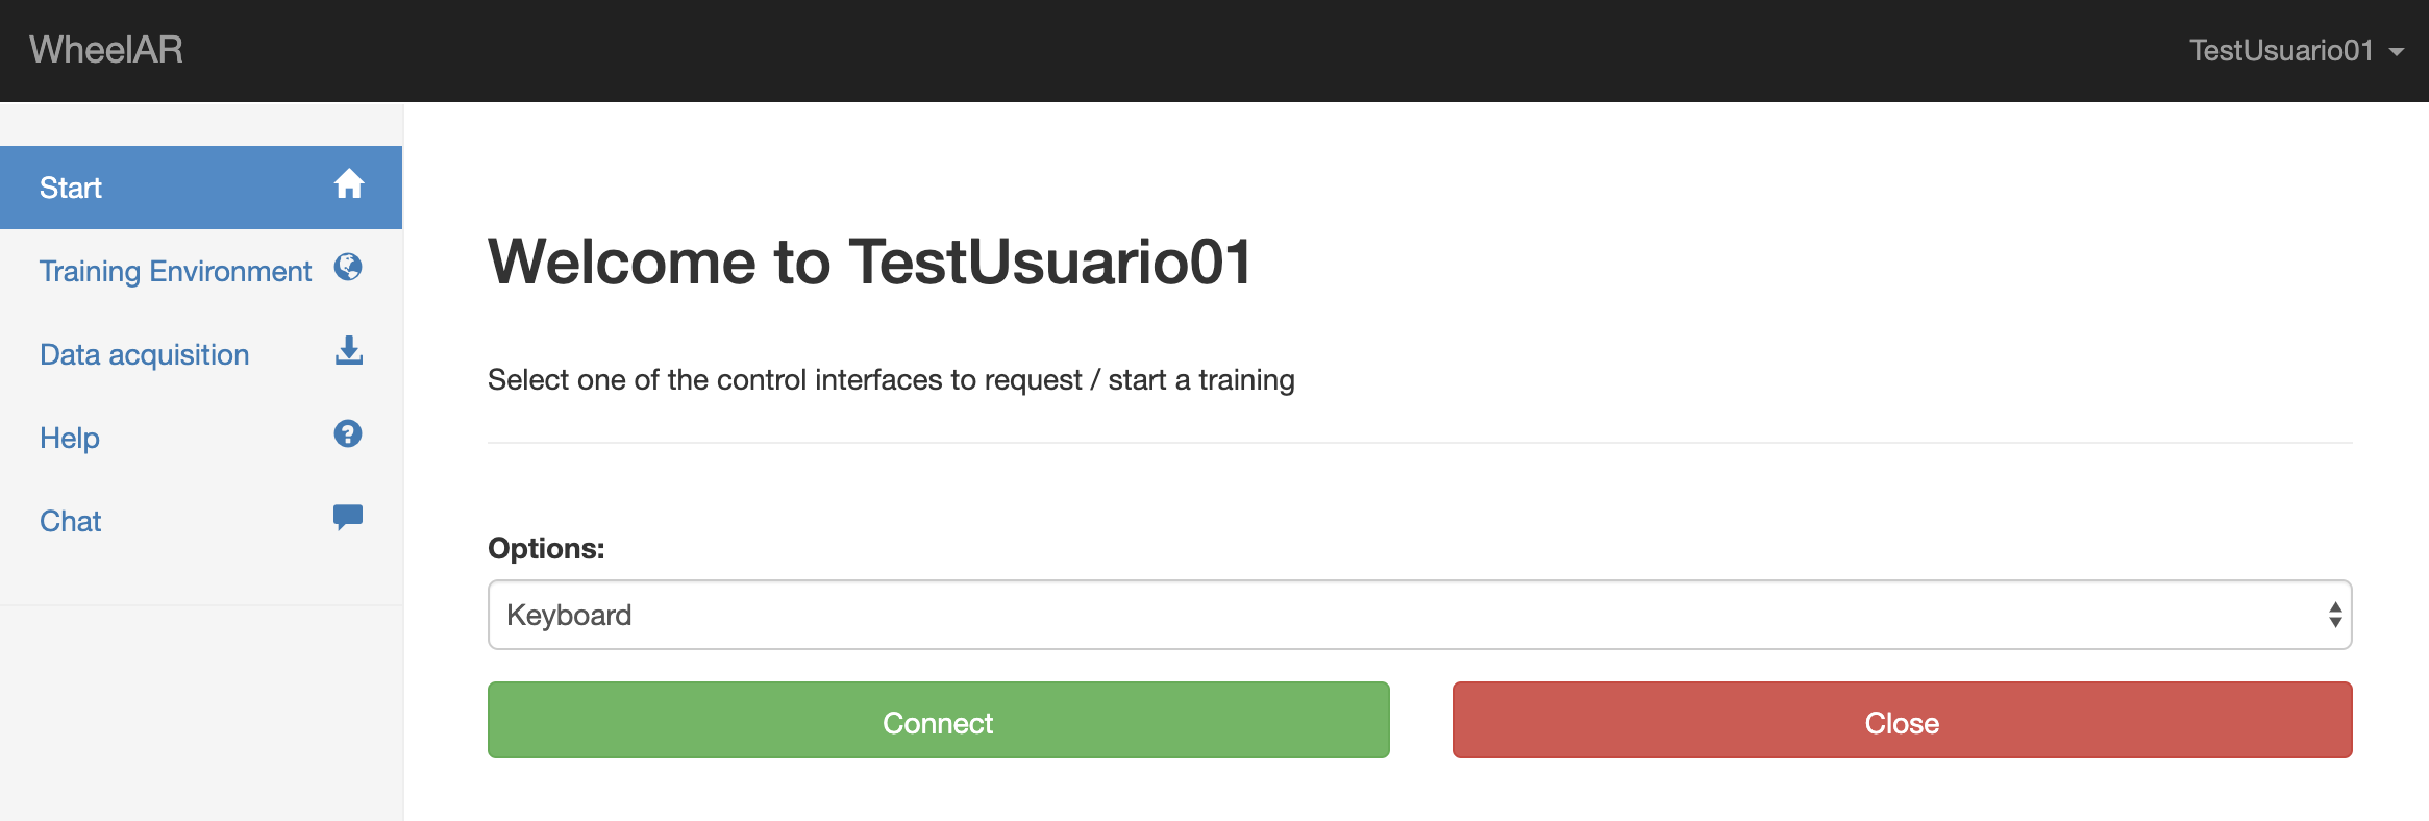
\includegraphics[width=1\linewidth]{img/apendiceD/tUserSession}
\caption{Main user page interaction} \label{fig:apDtUserSession}
\end{center}
\vspace{-15pt}
\end{figure}

If the ``Connect''  button is pressed, the user will be redirected to the ``Waiting page''  as presented in Figure \ref{fig:apDtWaitingSession}, until the Health professional, responsible for his process, releases the training environment. While the user is waiting, he has to read the 3D's models information (description and action) that might be chosen for his training. Then, his status will be updated to ``waiting''.

\begin{figure}[!hbt]
\begin{center}
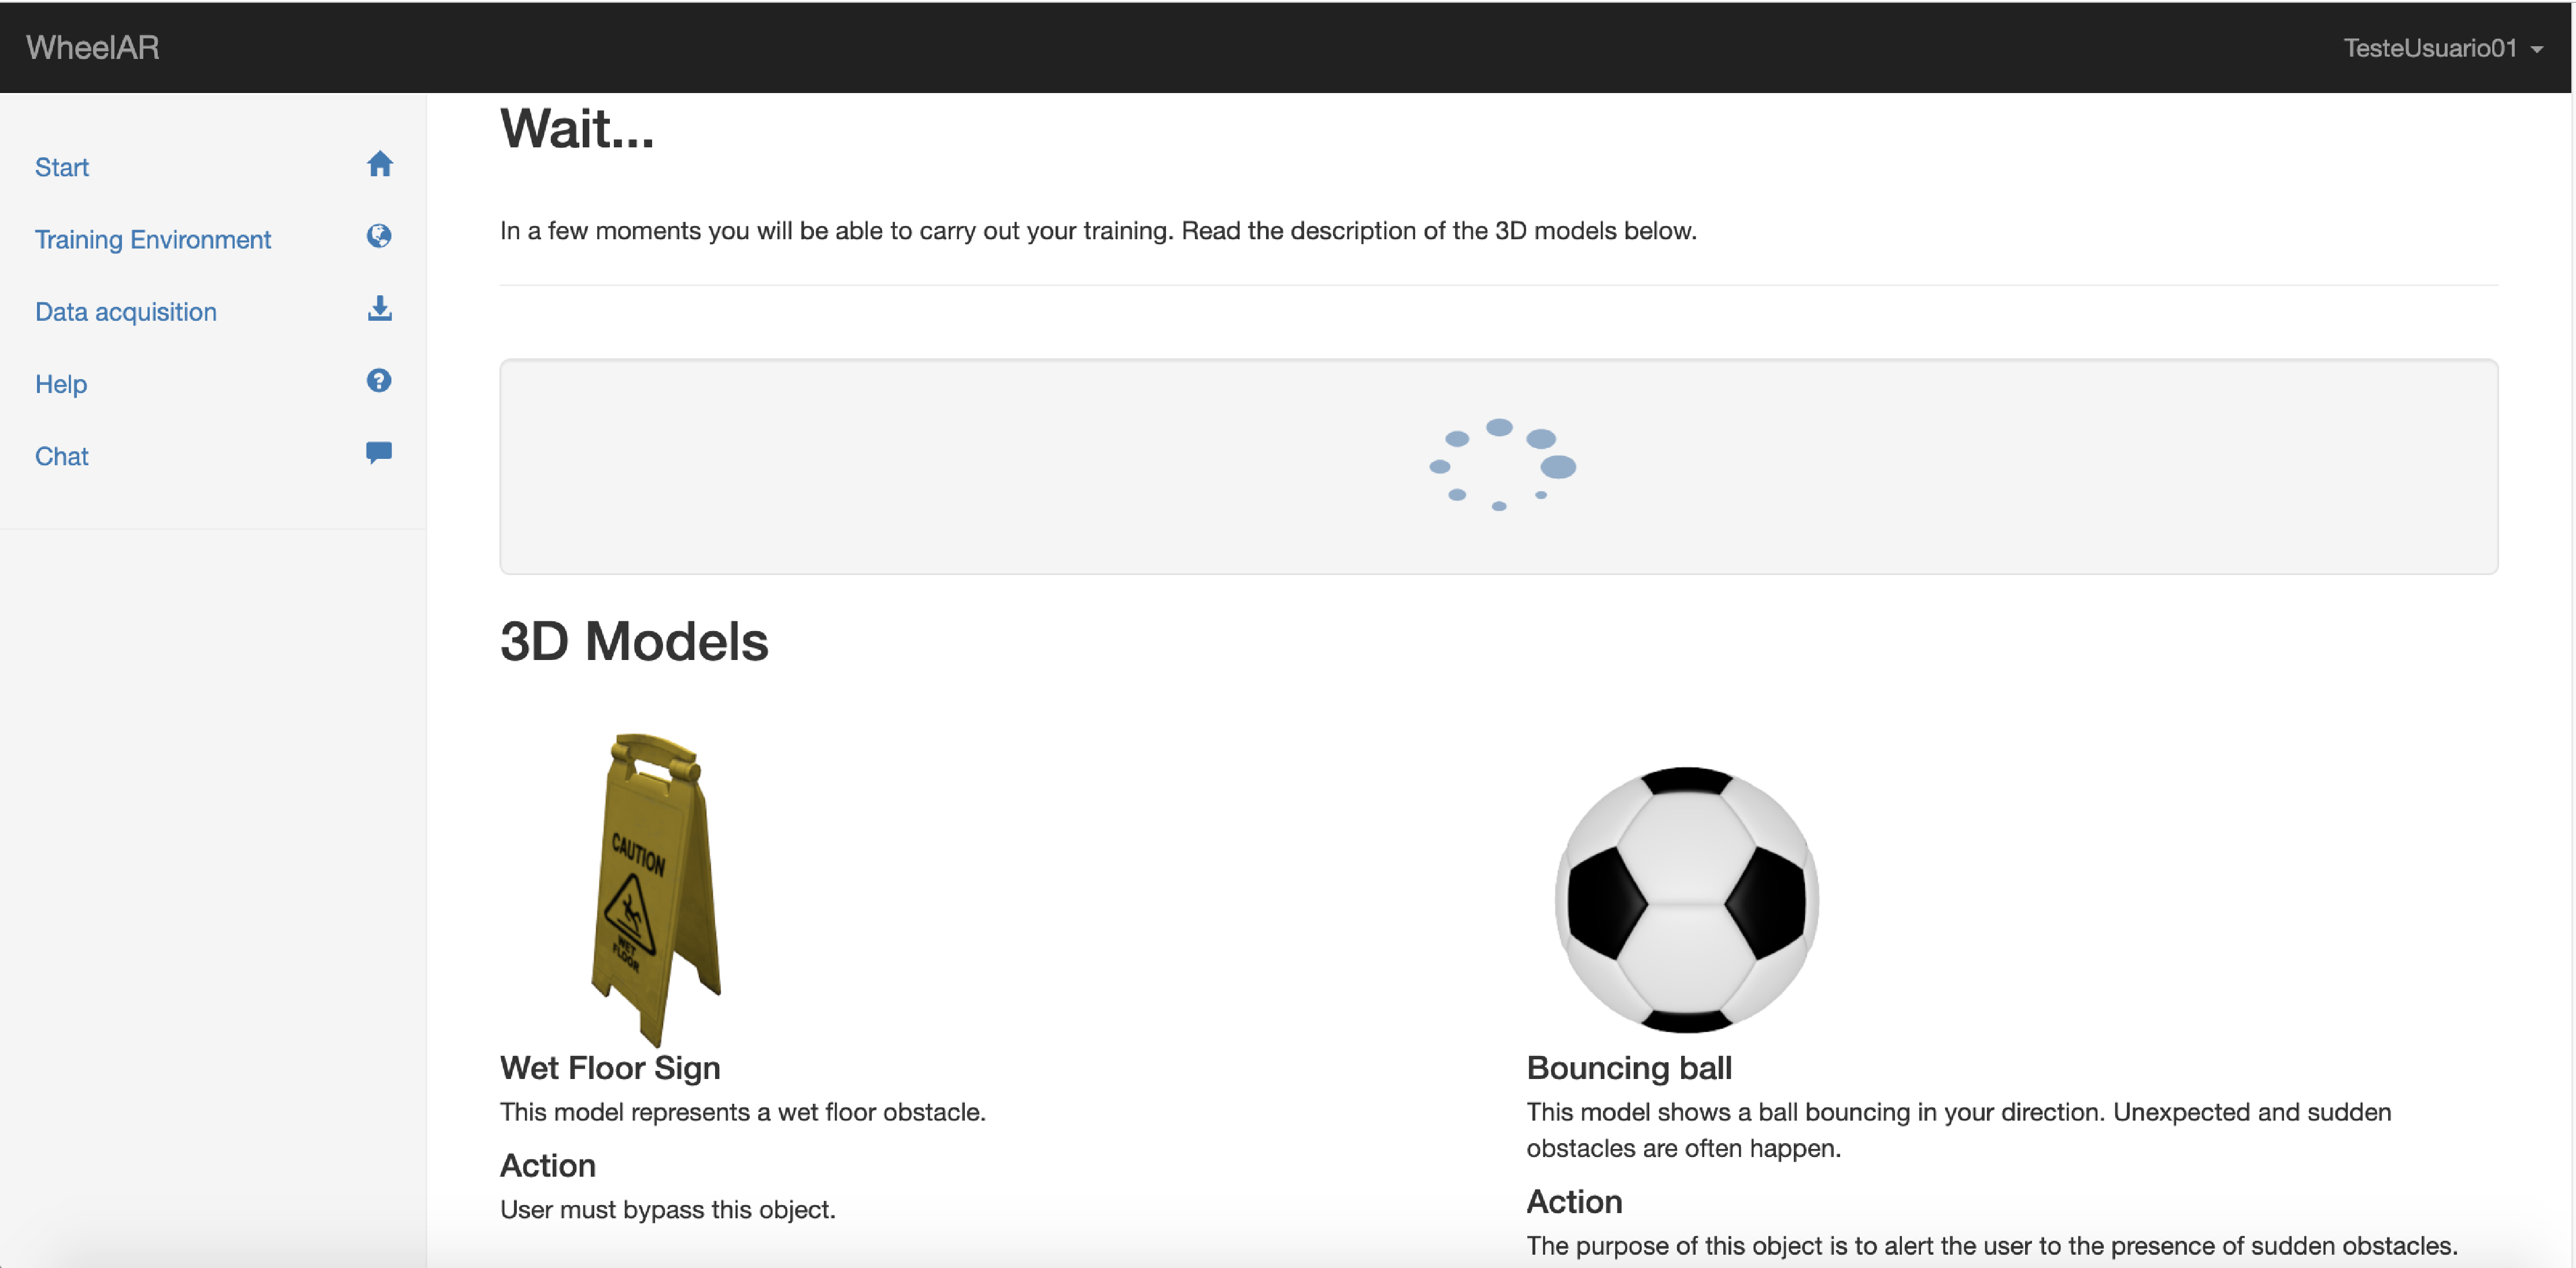
\includegraphics[width=1\linewidth]{img/apendiceD/tWaitingSession}
\caption{Waiting release training page} \label{fig:apDtWaitingSession}
\end{center}
\vspace{-15pt}
\end{figure}


\subsubsection{Data acquisition} 


Since a web browser is a sandbox application, to issue commands inputs to a remote PW, the user has to download the cross-platform Java$\texttrademark$ application shown in Figure \ref{fig:apDdataAcquisition01} and \ref{fig:apDdataAcquisition02}. From this application, a data connection with the command servlet is established. This servlet is responsible for forwarding all control input to the training environment. However, when a keyboard is used as an interface control, this application is not requested, because the browser recognizes the keyboard as basic input.  To start the data-flow, the user has to select an option If it is ``joystick''  then select the port and then press the button ``Connect''  or ``Disconnect'' to close data-flow and application. 

\begin{figure}[!htbp]
\center
\begin{minipage}{0.45\linewidth}
\center
\captionsetup{justification=centering,margin=0.5cm,font=tiny}
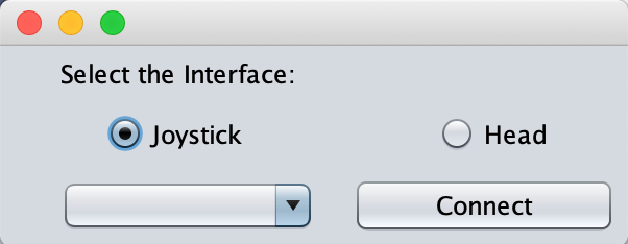
\includegraphics[width=1\linewidth]{img/apendiceD/dataAcquisition01}
\caption{Starting dataflow} \label{fig:apDdataAcquisition01}
\end{minipage}
\begin{minipage}{0.45\linewidth}
\center
\captionsetup{justification=centering,margin=0cm,font=tiny}
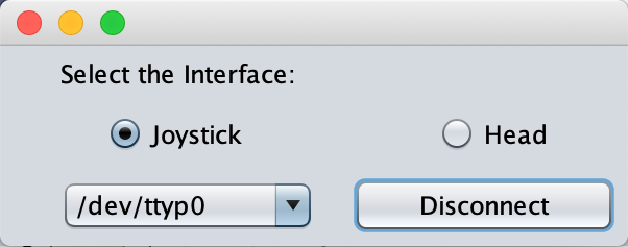
\includegraphics[width=1\linewidth]{img/apendiceD/dataAcquisition02}
\caption{Close dataflow} \label{fig:apDdataAcquisition02}
\end{minipage}
\end{figure}

\subsubsection{ViewPort} 

When the training session is released, the user status is changed to ``training''  and redirected to this page shown in Figure \ref{fig:apDtViewPortUser}, which provides a first-person experience view. 

\begin{figure}[!hbt]
\begin{center}
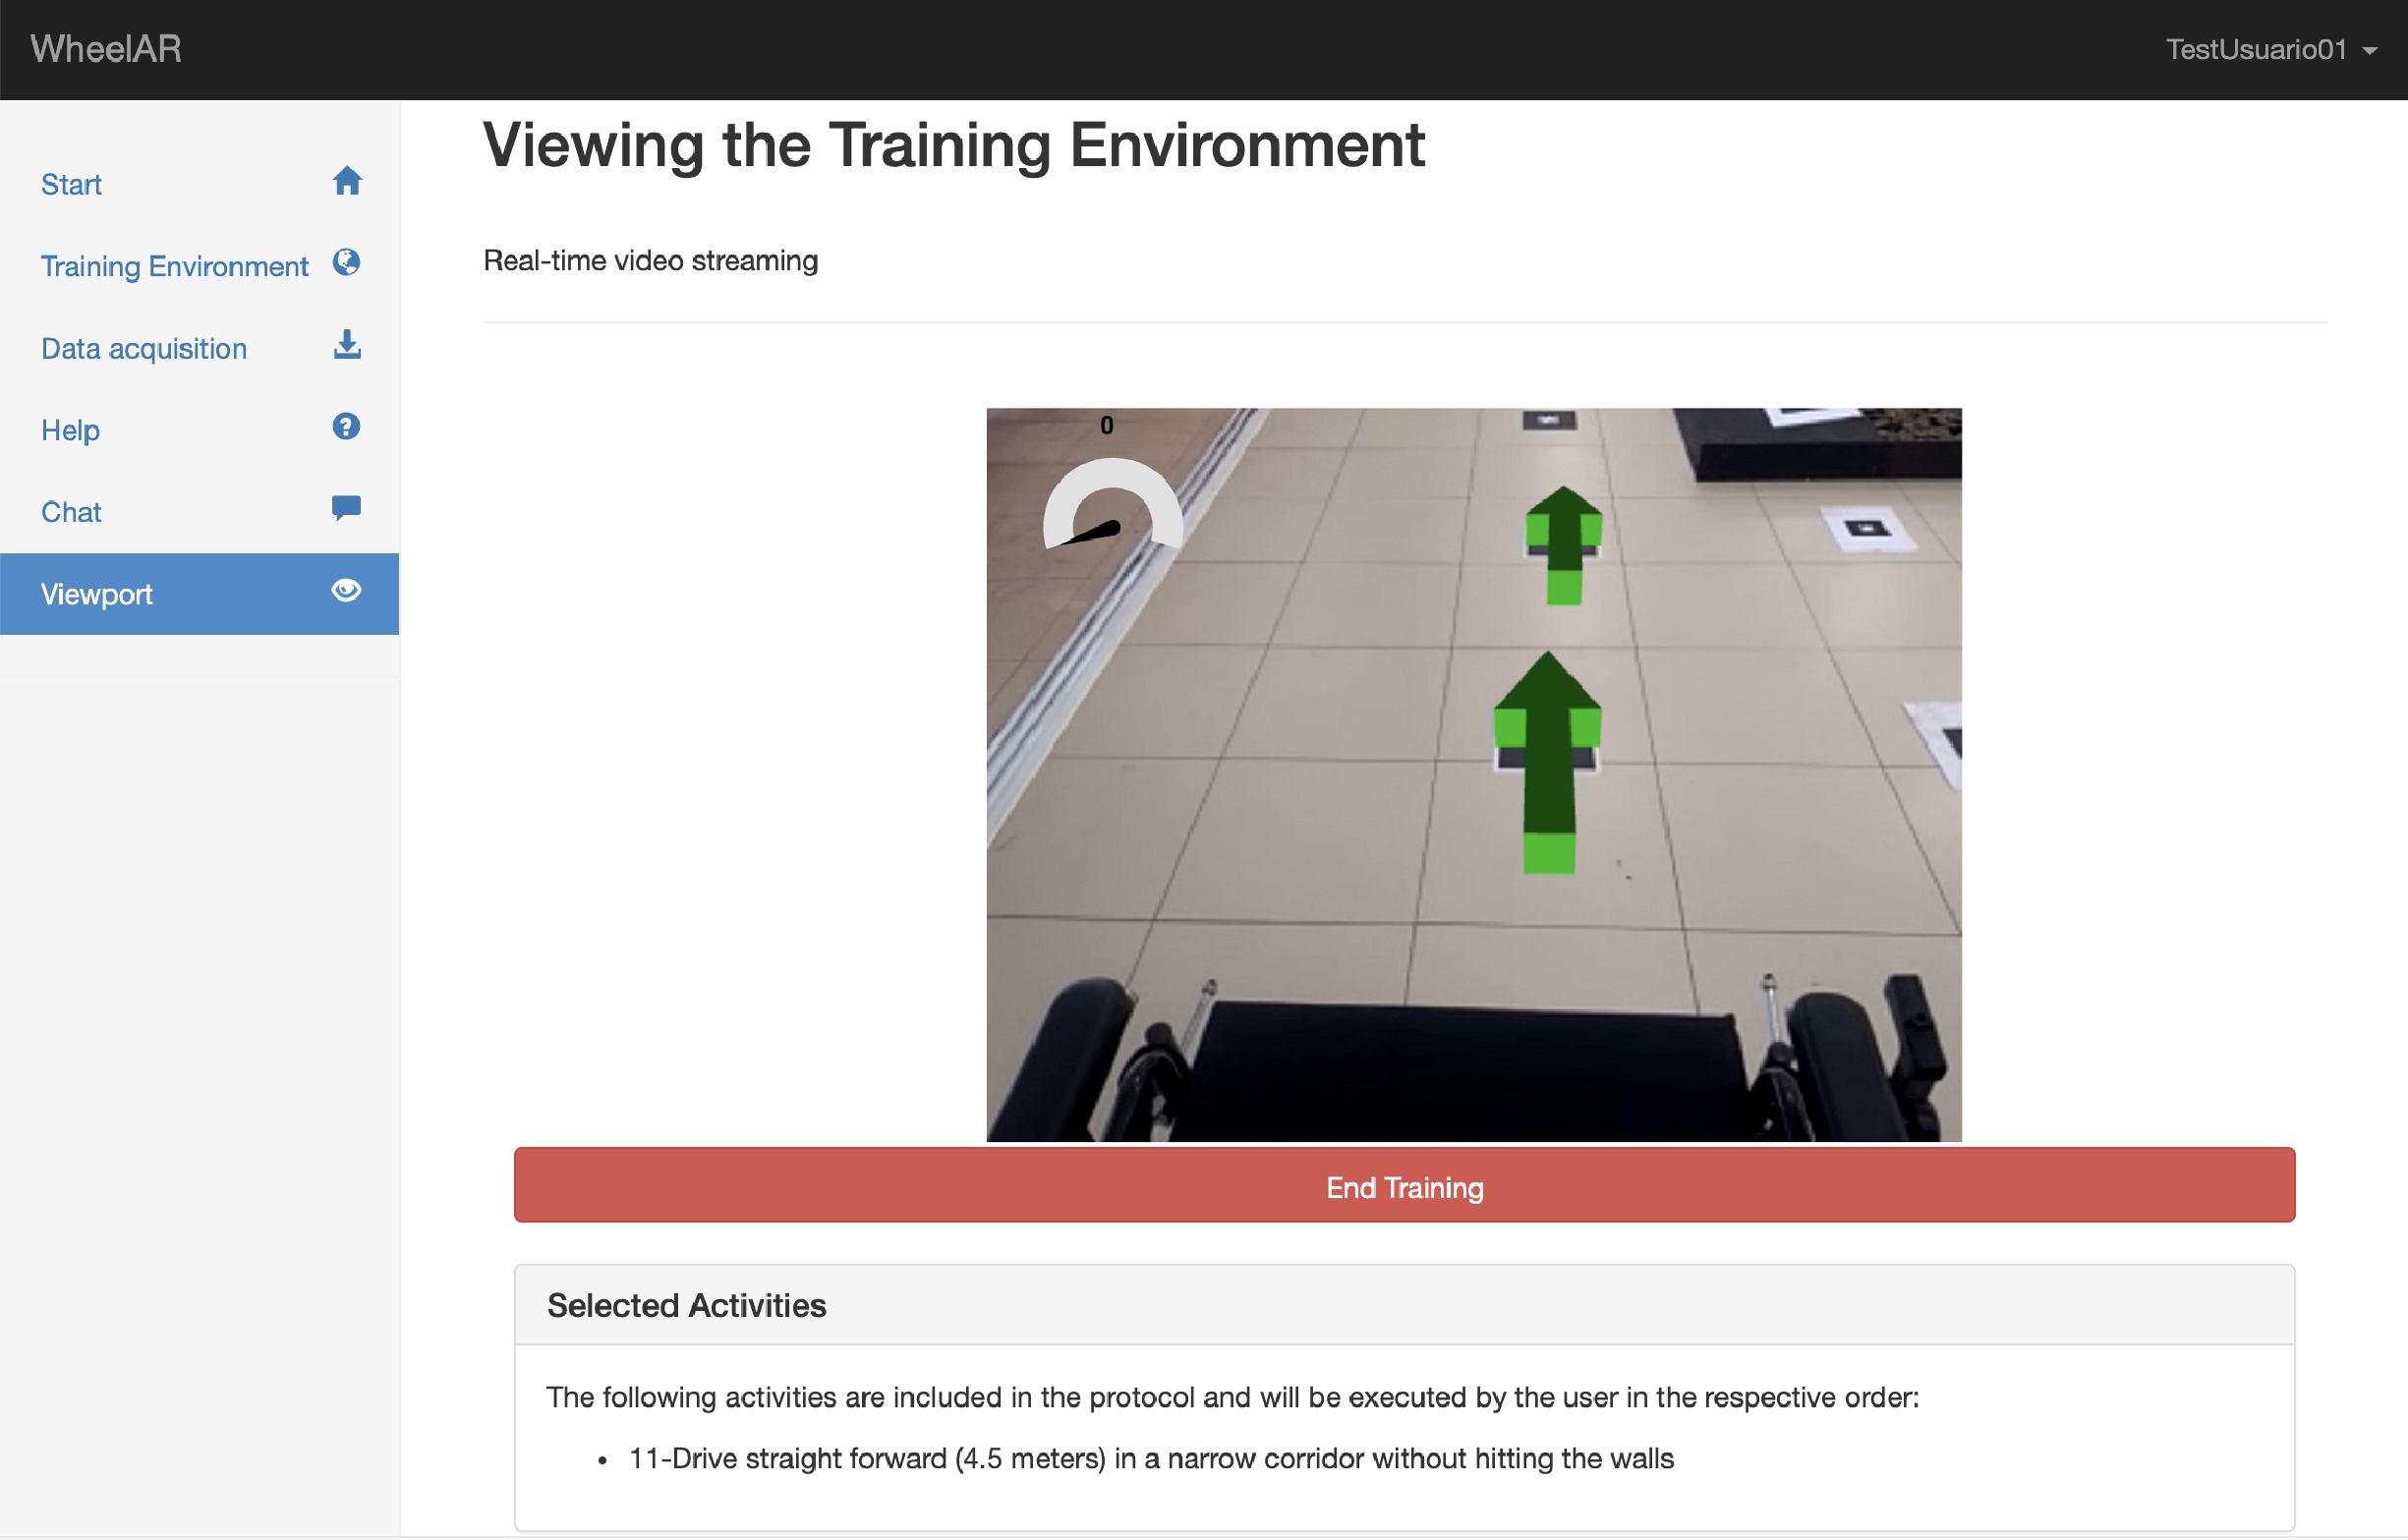
\includegraphics[width=1\linewidth]{img/apendiceD/tViewPortUser}
\caption{Real-time video streaming preview page} \label{fig:apDtViewPortUser}
\end{center}
\vspace{-15pt}
\end{figure}

The exercises prepared for each training protocol is listed on page bottom. The ``End training''  button has to be pressed when the training session has been concluded redirecting to the main users' page presented in Figure \ref{fig:apDtUserSession}, updating the user status to ``on-line''.


\section{Final considerations}

This chapter described all implementation details. In the next chapter, preliminaries results will be presented and discussed.